\documentclass[a4paper, 12pt]{report}

%---PREAMBLE BEGINS HERE---

% Use custom report style package
\usepackage{styles/report}

% Page headers and footers
\usepackage{fancyhdr}
\usepackage{array}
% Section formatting
\usepackage{titlesec}
\usepackage{fancyvrb}
% Graphics and figures
\usepackage{graphicx}
\usepackage{float}

% Code formatting
\usepackage{minted}
\usepackage{listings}

\lstdefinelanguage{JavaScript}{
  keywords={break,case,catch,class,const,continue,debugger,default,delete,do,else,export,extends,finally,for,function,if,import,in,instanceof,let,new,return,super,switch,this,throw,try,typeof,var,void,while,with,yield,async,await,of},
  sensitive=true,
  comment=[l]{//},
  morecomment=[s]{/*}{*/},
  morestring=[b]',
  morestring=[b]",
  morestring=[b]`
}

% Lists and enumerations
\usepackage{enumitem}

% Glossaries and acronyms
\usepackage[acronym, nomain, section=section]{glossaries}
\usepackage{glossaries-extra}

%  Required packages (add to your preamble if not already present):
   \usepackage{pgfplots}
    \pgfplotsset{compat=1.18}
    \usepackage{pgfplotstable}
    \usepackage{booktabs}
    \usepackage{multirow}
    \usepackage{colortbl}
    \usepackage{xcolor}
    \usepackage{tikz}
    \usetikzlibrary{patterns}
    \usepackage{subcaption}
    \usepackage{array}
    \usepackage{float}
% ─────────────────────────────────────────────────────────────────────────────
 
% ─── Colour palette ──────────────────────────────────────────────────────────
\definecolor{primary}{HTML}{2E75B6}
\definecolor{secondary}{HTML}{ED7D31}
\definecolor{accent}{HTML}{70AD47}
\definecolor{highlight}{HTML}{FFC000}
\definecolor{danger}{HTML}{C00000}
\definecolor{rowgray}{HTML}{F2F2F2}
\definecolor{headblue}{HTML}{D5E8F0}

\lstdefinestyle{appendixcode}{
  basicstyle=\ttfamily\footnotesize,
  breaklines=true,
  breakatwhitespace=false,
  columns=fullflexible,
  keepspaces=true,
  showstringspaces=false,
  frame=single,
  rulecolor=\color{primary},
  backgroundcolor=\color{rowgray},
  captionpos=b
}
 
% ─────────────────────────────────────────────────────────────────────────────

% Table of contents customization
\usepackage{tocloft}
\usepackage[nottoc]{tocbibind}
\hyphenpenalty=7000
\exhyphenpenalty=7000
\tolerance=1000
\emergencystretch=2em
\setlist[itemize]{noitemsep, topsep=0pt}
\setlist[enumerate]{noitemsep, topsep=0pt}

\newglossarystyle{acronyms}{%
  \renewenvironment{theglossary}{\begin{tabular}{ll}}{\end{tabular}}%
  \renewcommand*{\glossaryheader}{}%
  \renewcommand*{\glsgroupheading}[1]{}%
  \renewcommand*{\glossentry}[2]{\glsentryitem{##1}\glstarget{##1}{\glossentryname{##1}} & \glossentrydesc{##1}\tabularnewline}%
  \renewcommand*{\subglossentry}[3]{\glstarget{##2}{\glossentryname{##2}} & \glossentrydesc{##2}\tabularnewline}%
  \renewcommand*{\glsgroupskip}{}%
}

\makeglossaries

\newgeometry{
    top=1in,
    bottom=1in,
    inner=1.5in,
    outer=1in,
}

% Document metadata - UPDATE BEFORE COMPILING
\newcommand{\projectTitle}{RedSentinel: Transformer-Based Generation and Obfuscation of Context-Aware XSS Payloads}
\newcommand{\projectDate}{May, 2026}
\newcommand{\projectAuthors}{%
    Bipin Bhattarai (WRC078BCT009) \\[0.3cm]
    Seamoon Pandey (WRC078BCT035) \\[0.3cm]
    Sworup Bhandari (WRC078BCT046)%
}
\newcommand{\projectSupervisor}{Sudip Dahal}
\providecommand{\department}{}
\renewcommand{\department}{Department of Electronics and Computer Engineering}
\providecommand{\institution}{}
\renewcommand{\institution}{Paschimanchal Campus}
\providecommand{\university}{}
\renewcommand{\university}{Tribhuvan University, Institute of Engineering}

% Limit section numbering depth to 3 levels (chapter.section.subsection)
\setcounter{secnumdepth}{3}
% Limit TOC depth to 3 levels
\setcounter{tocdepth}{3}

\renewcommand{\cftfigpresnum}{Figure\ }
\setlength{\cftfignumwidth}{5em}

\renewcommand{\cfttabpresnum}{Table\ }
\setlength{\cfttabnumwidth}{4.5em}

\renewcommand{\contentsname}{TABLE OF CONTENTS}
\setlength{\cftbeforechapskip}{6pt}
\renewcommand{\cftchapaftersnum}{.}
\renewcommand{\cftchapleader}{\cftdotfill{\cftdotsep}}
\renewcommand{\cftchapfont}{\bfseries}

\renewcommand{\cfttoctitlefont}{\fontsize{12pt}{12pt}\bfseries}
\setlength{\cftbeforetoctitleskip}{0pt}
\setlength{\cftaftertoctitleskip}{12pt}

\renewcommand{\cftloftitlefont}{\fontsize{12pt}{12pt}\bfseries}
\setlength{\cftbeforeloftitleskip}{20pt}
\setlength{\cftafterloftitleskip}{20pt}

\renewcommand{\cftlottitlefont}{\fontsize{12pt}{12pt}\bfseries}
\setlength{\cftbeforelottitleskip}{20pt}
\setlength{\cftafterlottitleskip}{20pt}

% Hyperref setup - Must be near end of preamble
\hypersetup{
  pdfauthor={Bipin Bhattarai, Seamoon Pandey, Sworup Bhandari},
  pdftitle={\projectTitle},
  pdfsubject={Mid-Term Report - Final Year Project},
  pdfkeywords={XSS, Cross-Site Scripting, Machine Learning, Transformer, Security Testing, Payload Generation}
}

\title{\projectTitle}
\date{\projectDate}

\doublespacing % Line spacing for main content

%---PREAMBLE ENDS HERE---
\begin{document}
%---MAIN DOCUMENT BEGINS HERE---

% Cover page
\newgeometry{top=1in, bottom=1in, left=1.5in, right=1in}


\begin{titlepage}
{
  \thispagestyle{empty}
    \centering
    \normalsize
      
    
\includegraphics[width=1.3in]{figures/tu.png}\\
     {\fontsize{13}{16}\selectfont TRIBHUVAN UNIVERSITY}\\[0.15cm]
    {\fontsize{16}{20}\selectfont\bfseries INSTITUTE OF ENGINEERING}\\[0.15cm]
    {\fontsize{13}{16}\selectfont\bfseries PASHCHIMANCHAL CAMPUS}\\

    \vspace{1.5cm}
      {\fontsize{14}{18}\selectfont\bfseries
        \MakeUppercase \projectTitle
    }\\
    \vspace{1.5cm}
    
    {\fontsize{12}{16}\selectfont BY:}\\[0.1cm]
    
    {\fontsize{12}{16}\selectfont\bfseries
        \begin{tabular}{ll}
              BIPIN BHATTRAI & PAS078BCT009 \\[-0.3cm]
              SEAMOON PANDEY & PAS078BCT035 \\[-0.3cm]
              SWORUP BHANDARI & PAS078BCT046 \\
        \end{tabular}
    }\\
        \vspace{1.5cm}
    {\fontsize{11.5}{17}\selectfont
        A PROJECT REPORT SUBMITTED IN PARTIAL FULFILLMENT OF THE  REQUIREMENTS FOR THE BACHELOR'S DEGREE IN COMPUTER ENGINEERING
    }\\
     \vspace{1.5cm}
     {\fontsize{12}{16}\selectfont
        DEPARTMENT OF ELECTRONICS AND COMPUTER ENGINEERING\\[0.15cm]
        POKHARA, NEPAL
    }\\
    \vspace{1cm}
	 \projectDate\\
}
\end{titlepage}

\restoregeometry


% Front matter - Roman numerals
\onehalfspacing
\pagenumbering{roman}
\pagestyle{plain}
\setcounter{page}{2}
\textcolor{white}{a}\\[2.5cm]
\begin{center}
    {\fontsize{13}{16}\selectfont\bfseries LETTER OF APPROVAL}
\end{center}
 
\vspace{0.5cm}
 
\noindent
{\fontsize{12}{20}\selectfont
The undersigned certify that they have read and recommended to the Institute of
Engineering for acceptance, a project report entitled \textbf{`RedSentinel: Transformer-Based Generation and Obfuscation of
Context-Aware XSS Payloads'} submitted by \textbf{Bipin Bhattrai, Seamoon Pandey and Sworup Bhandari} in partial fulfillment of the requirements for the Bachelor's Degree in Computer Engineering.
}
 
\vspace{0.8cm}
 
% Supervisor
\noindent\rule{8cm}{0.4pt}\\[0.2cm]
{\fontsize{12}{16}\selectfont
Supervisor, \textbf{Asst. Prof. Sudip Dahal}\\
Department of Electronics and Computer Engineering\\
Institute of Engineering, Paschimanchal Campus
}
 
\vspace{0.8cm}
 
% External Examiner
\noindent\rule{8cm}{0.4pt}\\[0.2cm]
{\fontsize{12}{16}\selectfont
External Examiner, \textbf{Bidur Devkota, PhD}\\
Assistant Professor, Gandaki College of Engineering and Sciences\\
Gandaki province, Kaski
}
 
\vspace{0.8cm}
 
% Coordinator
\noindent\rule{8cm}{0.4pt}\\[0.2cm]
{\fontsize{12}{16}\selectfont
Coordinator, \textbf{Asst. Prof. Hom Nath Tiwari}\\
Head of Department\\
Department of Electronics and Computer Engineering\\
Institute of Engineering, Paschimanchal Campus
}
 
\vspace{0.8cm}
 
\begin{center}
    {\fontsize{12}{16}\selectfont DATE OF APPROVAL : 25 MAY 2026}
\end{center}
\include{includes/COPYRIGHT}
\chapter*{\MakeUppercase{ACADEMIC AND ETHICAL DECLARATION}} 
This report is written for academic analysis and defensive software engineering. The project domain is dual-use: an XSS scanner can support authorized vulnerability assessment, but the same technical knowledge may be misused against systems without permission. Accordingly, the report avoids operational instructions for unauthorized exploitation and frames payload generation,fuzzing, and browser verification as controlled defensive testing capabilities. Any implementation ordemonstration should be limited to owned systems, intentionally vulnerable labs, bug-bounty scopes, or environments where explicit written authorization exists. The evaluation in this report is based on repository evidence available through connected source inspection and selected external academic/security references. Repository evaluation claims are treated as project-provided evidence unless independently executed. The report therefore distinguishes between implemented code, documented behavior, and evaluation assertions.
% Acknowledgments
\chapter*{\MakeUppercase{Acknowledgments}}
\addcontentsline{toc}{chapter}{Acknowledgments}
We would like to express our sincere gratitude to everyone who contributed to the successful completion of this report and the development of the Red Sentinel project. We extend our deepest appreciation to our project supervisor, \textbf{Mr. Sudip Dahal}, for his invaluable guidance, continuous support, and constructive feedback throughout this research. His expertise in web security, machine learning, and computer networking has been instrumental in shaping the direction and quality of our work.

We would also like to thank the Department of Electronics and Computer Engineering at Tribhuvan University Pashchimanchal Campus for providing the essential resources, infrastructure, and academic environment that made this project possible.
\vspace{1cm}

\begin{flushright}
Bipin Bhattarai \\
Seamoon Pandey \\
Sworup Bhandari \\
\vspace{0.5cm}
\textit{May, 2026}
\end{flushright}

% Abstract
\chapter*{\MakeUppercase{Abstract}}
\addcontentsline{toc}{chapter}{Abstract}
Cross-Site Scripting (XSS) remains a persistent web vulnerability and traditional scanners, dependent on signatures and manually crafted payloads, struggle with modern filtering mechanisms and diverse injection contexts. The system employs a polyglot microservice architecture combining a TypeScript/NestJS orchestration core with three specialized Python-based AI microservices, all coordinated through a distributed job queue backed by Redis and surfaced via a real-time Next.js dashboard.

The core innovation lies in the integration of a fine-tuned DistilBERT transformer model for injection context classification, combined with a 59,122-entry labeled XSS payload dataset and a multistrategy payload mutation and obfuscation engine. This allows RedSentinel to reason about the semantic context of injection points, distinguishing HTML attribute contexts from JavaScript sink contexts, DOM-based sinks from server-reflected contexts, and generate payloads that are specifically crafted to survive filtering within that context.

The scanner performs an end-to-end pipeline consisting of optional target authentication, crawling, context analysis, payload generation, fuzzing, and report generation. Payload generation uses a curated payload bank of approximately 59,122 entries, mutation and obfuscation strategies, and XGBoost ranking when the trained ranker artifact is available, with heuristic fallback otherwise. The fuzzer checks reflection, supports DOM-oriented and stored-XSS paths with limitations, and can use headless browser verification to distinguish executable payloads from plain textual reflection

This report provides a comprehensive technical account of the system's architecture,module design, API contracts, dataset and model artifacts, scan pipeline, evaluation results and testing approach of RedSentinel.
\vspace{1cm}

\noindent\textbf{Keywords:} Cross-Site Scripting, XSS, Machine Learning, Transformer Models, Adversarial Payload Generation, Web Security, Automated Penetration Testing, Obfuscation, Context-Aware Attack Generation, BullMQ, Uvicorn, Pydantic, Playwright




% Table of Contents
\tableofcontents
\newpage

% List of Figures
\listoffigures
\vspace{1em}   % adjust as needed
\newpage
\listoftables
\newpage
% List of Tables (only if tables exist)

% List of Abbreviations
\chapter*{List of Abbreviations}
\addcontentsline{toc}{chapter}{List of Abbreviations}

\begin{description}
    \item[AI] Artificial Intelligence
    \item[API] Application Programming Interface
    \item[AWS] Amazon Web Services
    \item[CI/CD] Continuous Integration/Continuous Deployment
    \item[CVE] Common Vulnerabilities and Exposures
    \item[DDQN] Double Deep Q-Network
    \item[DOM] Document Object Model
    \item[DQN] Deep Q-Network
    \item[DVWA] Damn Vulnerable Web Application
    \item[GRU] Gated Recurrent Unit
    \item[HTML] HyperText Markup Language
    \item[LSTM] Long Short-Term Memory
    \item[ML] Machine Learning
    \item[mTLS] Mutual Transport Layer Security
    \item[NLP] Natural Language Processing
    \item[OWASP] Open Web Application Security Project
    \item[RL] Reinforcement Learning
    \item[RNN] Recurrent Neural Network
    \item[WAF] Web Application Firewall
    \item[XSS] Cross-Site Scripting
\end{description}

\newpage

% Main content - Arabic numerals
\pagenumbering{arabic}
\pagestyle{plain}

% Chapters
\chapter{Introduction}
\section{Background}
RedSentinel is an AI-augmented web application security scanner purpose-built to detect Cross-Site Scripting (XSS) vulnerabilities. XSS remains one of the most persistently exploited vulnerability classes in modern web applications. According to the OWASP Top 10, injection-related vulnerabilities have appeared consistently across multiple editions of the industry-standard web application risk rankings, with Cross-Site Scripting discussed within A03:2021 (Injection) as a prominent client-side security concern \cite{owasp_top10_2021}. The widespread prevalence of XSS is further corroborated by the Common Vulnerabilities and Exposures (CVE) database, where XSS routinely accounts for a substantial share of annually reported web vulnerabilities \cite{mitre_cve}.

Traditional XSS scanners operate on static, manually curated payload lists paired with simple string-matching heuristics. While adequate for detecting trivial reflections, these approaches fail in two important respects: they are blind to injection context meaning they cannot distinguish between a parameter reflected inside a JavaScript string literal and one reflected inside an HTML attribute value, contexts that demand entirely different payload structures and they are easily defeated by modern Web Application Firewalls (WAFs), which signature-match against known payload patterns \cite{bau2010state}.

RedSentinel addresses both limitations through a five-phase pipeline that integrates machine learning-based injection context classification at the core of its analysis workflow. The context classification is performed by a fine-tuned DistilBERT model, a distilled variant of the BERT transformer architecture, introduced by Devlin et al.\cite{devlin2019bert} and subsequently compressed by Sanh et al.\cite{sanh2019distilbert} to approximately 40\% of BERT's parameter count while retaining 97\% of its language understanding capability on the GLUE benchmark. The model is fine-tuned on a domain-specific dataset of 59,122 labeled XSS payloads, enabling it to classify injection contexts (HTML body, HTML attribute, JavaScript string, JavaScript code block, URL context, CSS context, and DOM sink) from source code fragments surrounding the injection point.

The system's architecture follows a polyglot microservices pattern. A NestJS/TypeScript orchestration core \cite{nestjs} manages the HTTP API, WebSocket real-time event streaming via Socket.io \cite{socketio}, job queue scheduling via BullMQ backed by Redis \cite{bullmq}, and PostgreSQL persistence via TypeORM \cite{typeorm}. Three independently deployable Python FastAPI microservices \cite{fastapi} handle the AI-intensive concerns: context analysis (port 5001), payload generation with mutation and obfuscation (port 5002), and HTTP/headless-browser fuzzing via Playwright \cite{playwright} (port 5003). Asynchronous job execution through BullMQ ensures the REST API remains non-blocking while scans execute in background workers, and Socket.io WebSocket events deliver real-time progress and vulnerability findings to the Next.js dashboard \cite{nextjs}.

The payload generation subsystem draws on a curated bank of 59,122 labeled XSS payloads. Payload selection is context-aware and WAF-evasion-weighted, followed by a mutation engine that applies systematic transformations (case variation, Unicode and HTML entity encoding, whitespace manipulation, and event-handler alternation) and an obfuscation layer that applies higher-order JavaScript transforms such as Base64/atob encoding, String.fromCharCode construction, and eval indirection. This approach is consistent with established research on WAF bypass techniques, which demonstrates that encoding diversity and structural variation significantly reduce detection rates of signature-based filters \cite{bau2010state}.

Vulnerability confirmation in the fuzzing phase employs a two-stage verification strategy: HTTP response reflection analysis followed by headless Chromium execution via Playwright, using a canary window property injection technique to confirm actual JavaScript execution rather than mere textual reflection. This dual-verification approach is aligned with best practices in automated XSS confirmation research, which distinguishes passive reflection (a necessary but insufficient condition for XSS) from confirmed execution. The system concludes each scan by generating vulnerability reports in HTML, PDF (via Puppeteer \cite{puppeteer}), and JSON formats, suitable for both human review and CI/CD pipeline integration.

\section{ Problem Statement}
Although XSS scanners and WAFs can identify many basic vulnerabilities, they often depend on static payloads and basic reflection checks, making them less effective at handling different injection contexts, WAF/filter bypasses, browser execution verification, and structured reporting.

\section{ Objectives}
The primary objectives of the RedSentinel are:
\begin{enumerate}[itemsep=2pt, topsep=-15pt]
    \item To design and implement RedSentinel, an AI-assisted, context-aware XSS scanner that crawls targets, analyses injection contexts, generates and ranks payloads, fuzzes and verifies vulnerabilities.
    \item To generate structured, actionable vulnerability reports in multiple formats.
\end{enumerate}

\chapter{Literature Review }
\section{Related Works}
The following review examines significant advancements in automated web security testing, with a particular focus on XSS payload generation and adversarial input synthesis. Existing research covers a wide spectrum of techniques, including reinforcement learning, neural machine translation, generative adversarial models, and transformer-based language approaches. By analysing these contributions, this review highlights the methodological trends, strengths, and limitations that shape for the design and development of the Red Sentinel system..

Foley and Maffeis (2022) propose HAXSS, a hierarchical reinforcement-learning framework to automatically generate XSS attack payloads. Their approach frames the payload creation as two nested RL ``games.'' The first agent learns to escape the immediate HTML context of user output (escaping tags or attributes), while the second agent intervenes whenever the application attempts sanitization, it learns to obfuscate the payload to bypass filters. Successful obfuscations are fed back into the first agent for further refinement. Implemented as an end-to-end black-box fuzzer, HAXSS was evaluated on both synthetic benchmarks and real web applications. It identified 131 XSS vulnerabilities (20\% more than state-of-the-art scanners) with zero false positives, including rediscovering known CVEs and uncovering 5 novel CVEs in production-grade sites. Thus, HAXSS demonstrates that hierarchical RL can produce diverse, context- and filter-aware payloads that significantly improve XSS discovery over traditional scanners \cite{foley2022haxss}.

Khan (2024) presents LL-XSS, an end-to-end deep generative model for crafting XSS payloads. Unlike hand-crafted or brute-fuzzed payloads, LL-XSS leverages a combination of auto-regressive neural networks and transformer architectures to analyze both frontend and backend web code and produce candidate attack scripts. The model is trained on example web application code to learn common injection patterns, then generates new malicious scripts aimed at identified vulnerabilities. In evaluation on the OWASP Juice Shop, the author reports that LL-XSS can automatically generate syntactically valid and exploitable XSS payloads by understanding the target's code context. This approach effectively automates the penetration-testing process: LL-XSS bypasses known filters and exposes vulnerabilities with minimal human guidance, demonstrating the promise of AI-driven payload creation for web security \cite{khan2024llxss}.

Frempong et al. (2021) developed HIJaX, a neural machine translation model that converts natural-language attack descriptions into working XSS payloads. The system was trained on paired examples of intent phrases and JavaScript exploits. Their experiments showed that the model could reliably generate valid payloads that triggered real XSS vulnerabilities, demonstrating that neural translation methods can automate exploit creation even for users with limited technical expertise \cite{frempong2021hijax}.

Pala et al. (2023) examined contemporary XSS scanners and highlighted XSStrike as a tool that combines intelligent fuzzing with basic machine-learning techniques. XSStrike analyzes the structure of a web page to detect injection points and then mutates payloads based on contextual feedback. Their evaluation showed that this approach improves detection and execution of XSS payloads across different contexts, illustrating the value of context-aware fuzzing \cite{pala2023xssassessment}.

Fink (2018) introduced FOXSS, a scanner that integrates static data-flow analysis with targeted, context-sensitive fuzzing. The tool identifies potential input flows and generates tailored payloads for each sink, verifying results in a real browser. FOXSS demonstrated very high detection accuracy, outperforming conventional scanners and significantly reducing false positives, indicating that program analysis combined with adaptive fuzzing can greatly enhance XSS detection \cite{fink2018foxss}.

Song et al. (2023) presented a grey-box fuzzing system that uses reinforcement learning to create and refine XSS payloads. After mapping all input points through static analysis, the authors trained RL agents (DQN, DDQN, and Policy Gradient) to adjust payloads based on execution feedback. The RL-based fuzzer identified all known XSS vulnerabilities in benchmark applications with no false positives, demonstrating that RL can effectively adapt payloads to complex contexts\cite{song2023greybox}.

Miczek et al. (2025) explored the use of large language models to generate obfuscated XSS attacks capable of evading machine-learning detectors. Their study showed that classifiers trained on standard payloads performed poorly when encountering obfuscated variants. By fine-tuning a transformer to generate diverse obfuscations, the authors significantly improved detector robustness after retraining. This work highlights the usefulness of LLM-generated adversarial examples for strengthening defensive models\cite{miczek2025llml_xss}.
\chapter{Methodology}

\section{Architectural Design Overview}

Red Sentinel is implemented using a microservice architecture. In this design, each major functional component of the system runs as an independent service. These services communicate via well-defined APIs and are coordinated by a central orchestration core the "Core Module." This microservice approach ensures that each module is isolated, independently deployable, testable, and can be scaled or replaced without impacting the rest of the system addressing concerns of maintainability, modularity, and system complexity typical in security tools.



\begin{figure}[H]
    \centering
    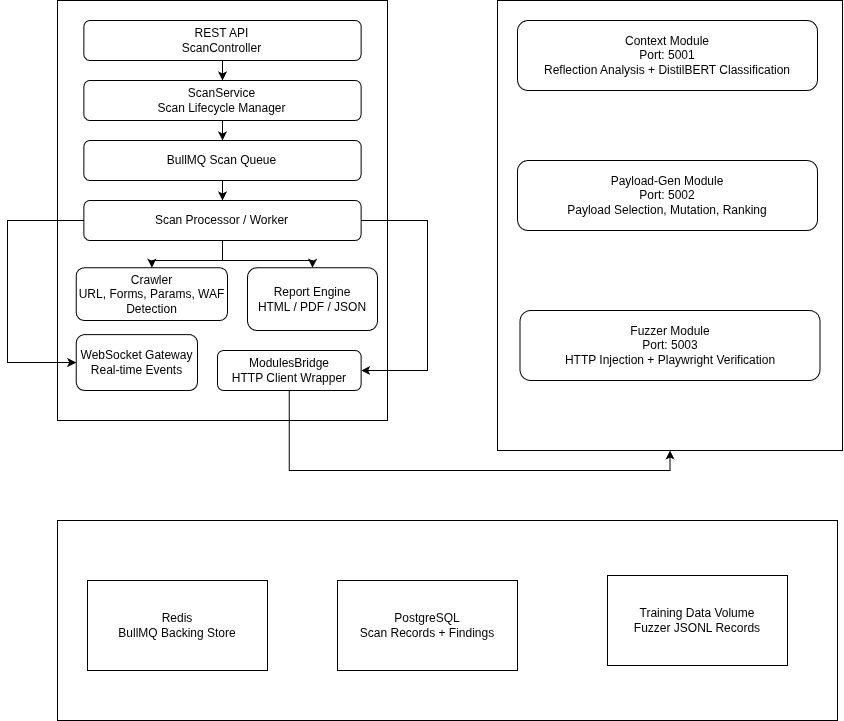
\includegraphics[width=1\linewidth]{figures/arch.png}
    \caption{System Architecture Diagram}
    \label{fig:system_architecture}
\end{figure}

The architecture consists of six primary services: a NestJS core service providing the REST API, WebSocket gateway, and job queue processor; three Python FastAPI microservices (Context, Payload-Gen, Fuzzer); a Next.js dashboard; and two infrastructure services (Redis and PostgreSQL).

\subsection{Design Principles}
\subsubsection{Separation of Concerns}

Each microservice is responsible for a single phase of the scanning pipeline. The Context module understands the injection context, the Payload Generation module understands payload selection and mutation, the Fuzzifier module understands HTTP-level injection and browser verification. The Core co-ordinates these phases without containing their implementation logic. This separation allows each service to be modified independently and be tested in isolation.

\subsubsection{Asynchronous Job Processing}
Scan jobs are not processed synchronously in the HTTP request-response cycle. When a client submits a POST /scan request, the Core immediately persists the scan record to PostgreSQL, enqueues a BullMQ job, and returns the scan ID to the client. The actual scanning pipeline executes asynchronously in a BullMQ worker process. This design decouples request handling from compute intensive scanning, allows multiple scans to be queued without blocking, and supports scan cancellation, retries, and priority management.

\subsubsection{Event-Driven Real-Time Updates}

The BullMQ scan processor emits events at each pipeline phase transition and upon each vulnerability discovery. These events are relayed to the NestJS WebSocket Gateway, which broadcasts them to subscribed Socket.io clients. This event-driven architecture provides clients with sub-second latency updates without polling.

\subsubsection{Health-Check Dependency Management}

Docker Compose service startup is conditioned on health checks: the Core service will not start until Redis, PostgreSQL, and all three Python microservices report healthy. Each Python service exposes a /health endpoint returning service status and model load state. This prevents race conditions during cold starts where the Core might attempt to call Python services before their AI models have loaded.

\subsection{Data Flow in Scan Execution}
A complete scan execution follows this data flow:
\begin{enumerate}[itemsep=2pt, topsep=-15pt]
    \item Client submits POST /scan with target URL, scan depth, and options.
    \item ScanController validates request, persists ScanRecord to PostgreSQL with status PENDING, enqueues BullMQ job with scan ID.
    \item  BullMQ Processor picks up job, updates status to RUNNING, begins Phase 1: CRAWL.
    \item Crawler spiders target URL up to configured depth, collecting all discovered URLs, query parameters, form fields, headers, and cookies. WAF detection heuristics run concurrently.
    Example:
      \begin{Verbatim}[fontsize=\scriptsize]
       Dicovered page:
        <script>
            var searchTerm = "USER_INPUT";
          </script>

                    Crawler output:
                    {
              "url": "https://demo-app.com/search?q=test",
              "parameter": "q",
              "reflectionPoint": "script_tag"}
      \end{Verbatim}
    \item Crawler results are passed to ModulesBridge, which issues POST /analyze to Context module (:5001).
    \item Context module probes each injection point with probe strings, analyzes reflections, and classifies each injection point's context using DistilBERT.
    \item Context classification results are passed to ModulesBridge, which issues POST /generate to Payload-Gen module (:5002).
    \item Payload-Gen module selects candidates from the dataset filtered by context, applies mutation and obfuscation, ranks payloads using a secondary ranker model.
     Example:
      \begin{Verbatim}[fontsize=\scriptsize]
       {
          {    "payloads": [
                "\";alert(1);//",
                "\"};alert(document.domain);//",
               ..........
              ]
            }
      \end{Verbatim}
    \item Ranked payloads are passed to ModulesBridge, which issues POST /fuzz to Fuzzer module (:5003).
    \item  Fuzzer injects payloads, checks HTTP responses for reflection, launches Playwright headless browser for verification of apparent reflections. Confirmed executions are reported as vulnerabilities.  Example:
      \begin{Verbatim}[fontsize=\scriptsize]
       {
          Injected response:
                <script>
        var searchTerm = "";alert(1);//";
      </script>
            }
      \end{Verbatim}
    \item Report Engine generates HTML/PDF/JSON reports. Scan status is set to COMPLETED. scan:complete WebSocket event is broadcast.
\end{enumerate}
\newpage
\begin{figure}[h]
  \centering
  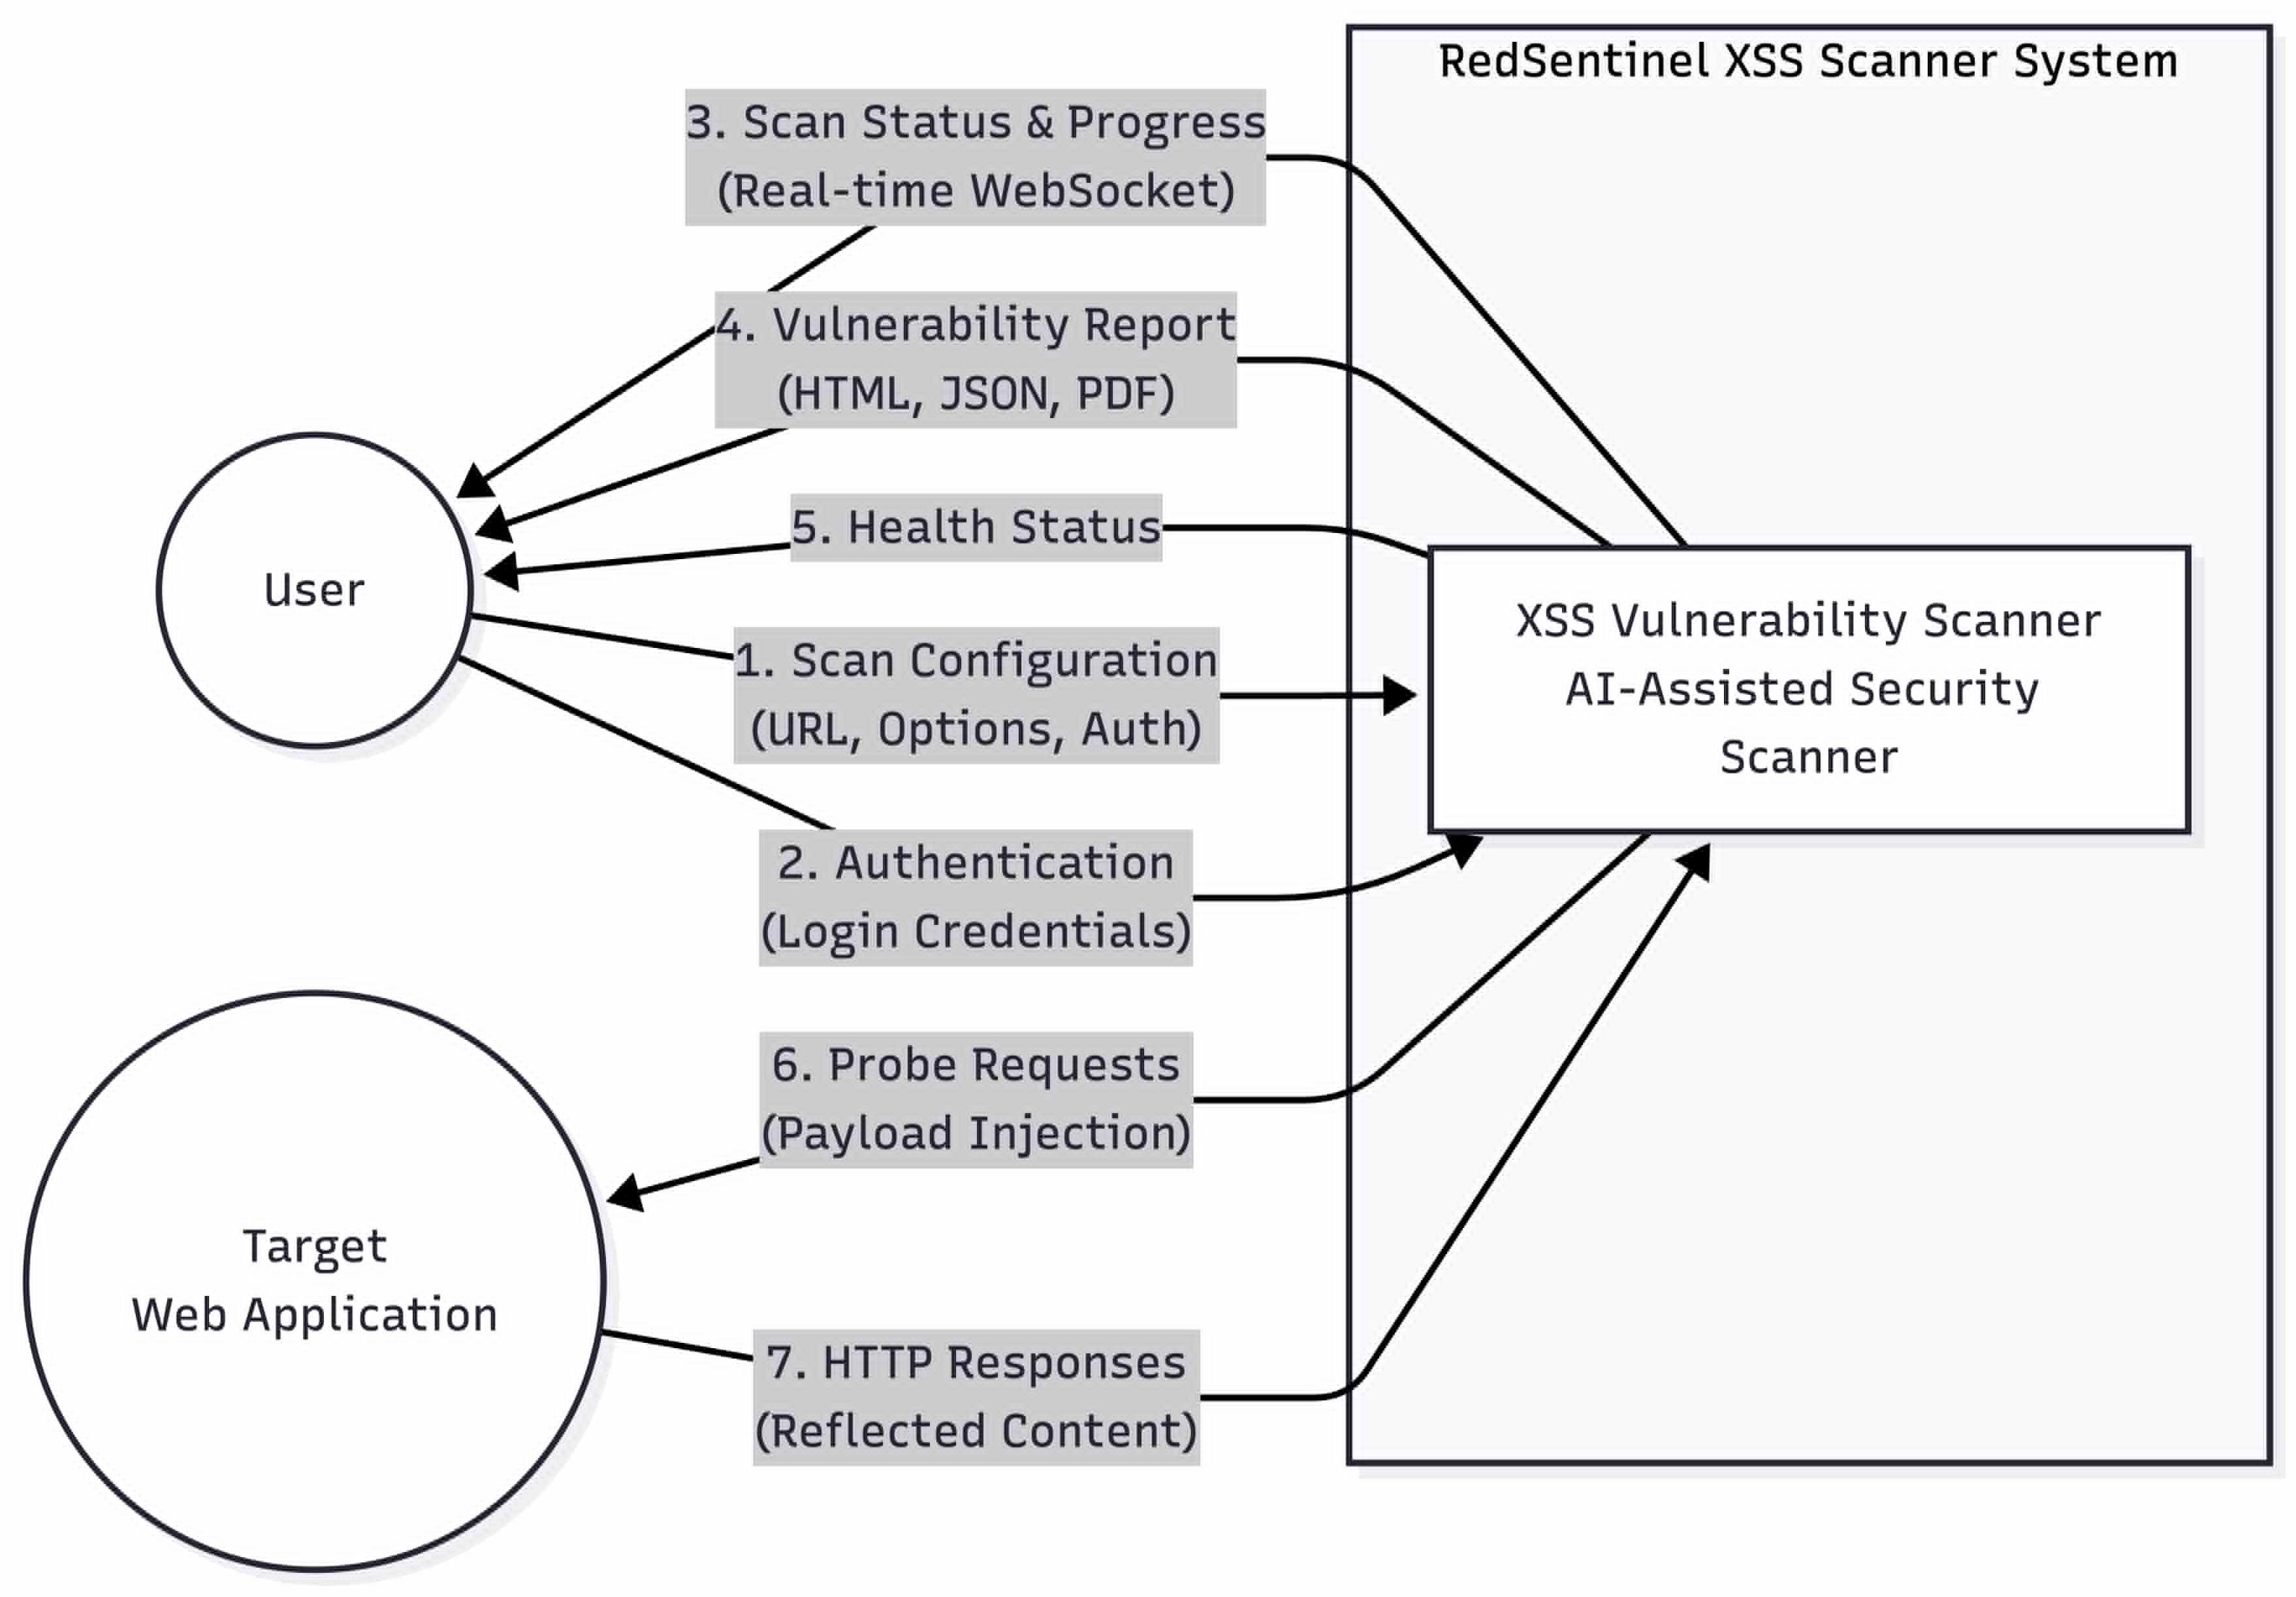
\includegraphics[width=0.8\textwidth]{figures/DFD0.jpg}
  \caption{High-Level Architecture and Communication Flow of the RedSentinel AI-Assisted XSS Vulnerability Scanner System.}
  \label{fig:example_image}
\end{figure}

\begin{figure}[H]
  \centering
  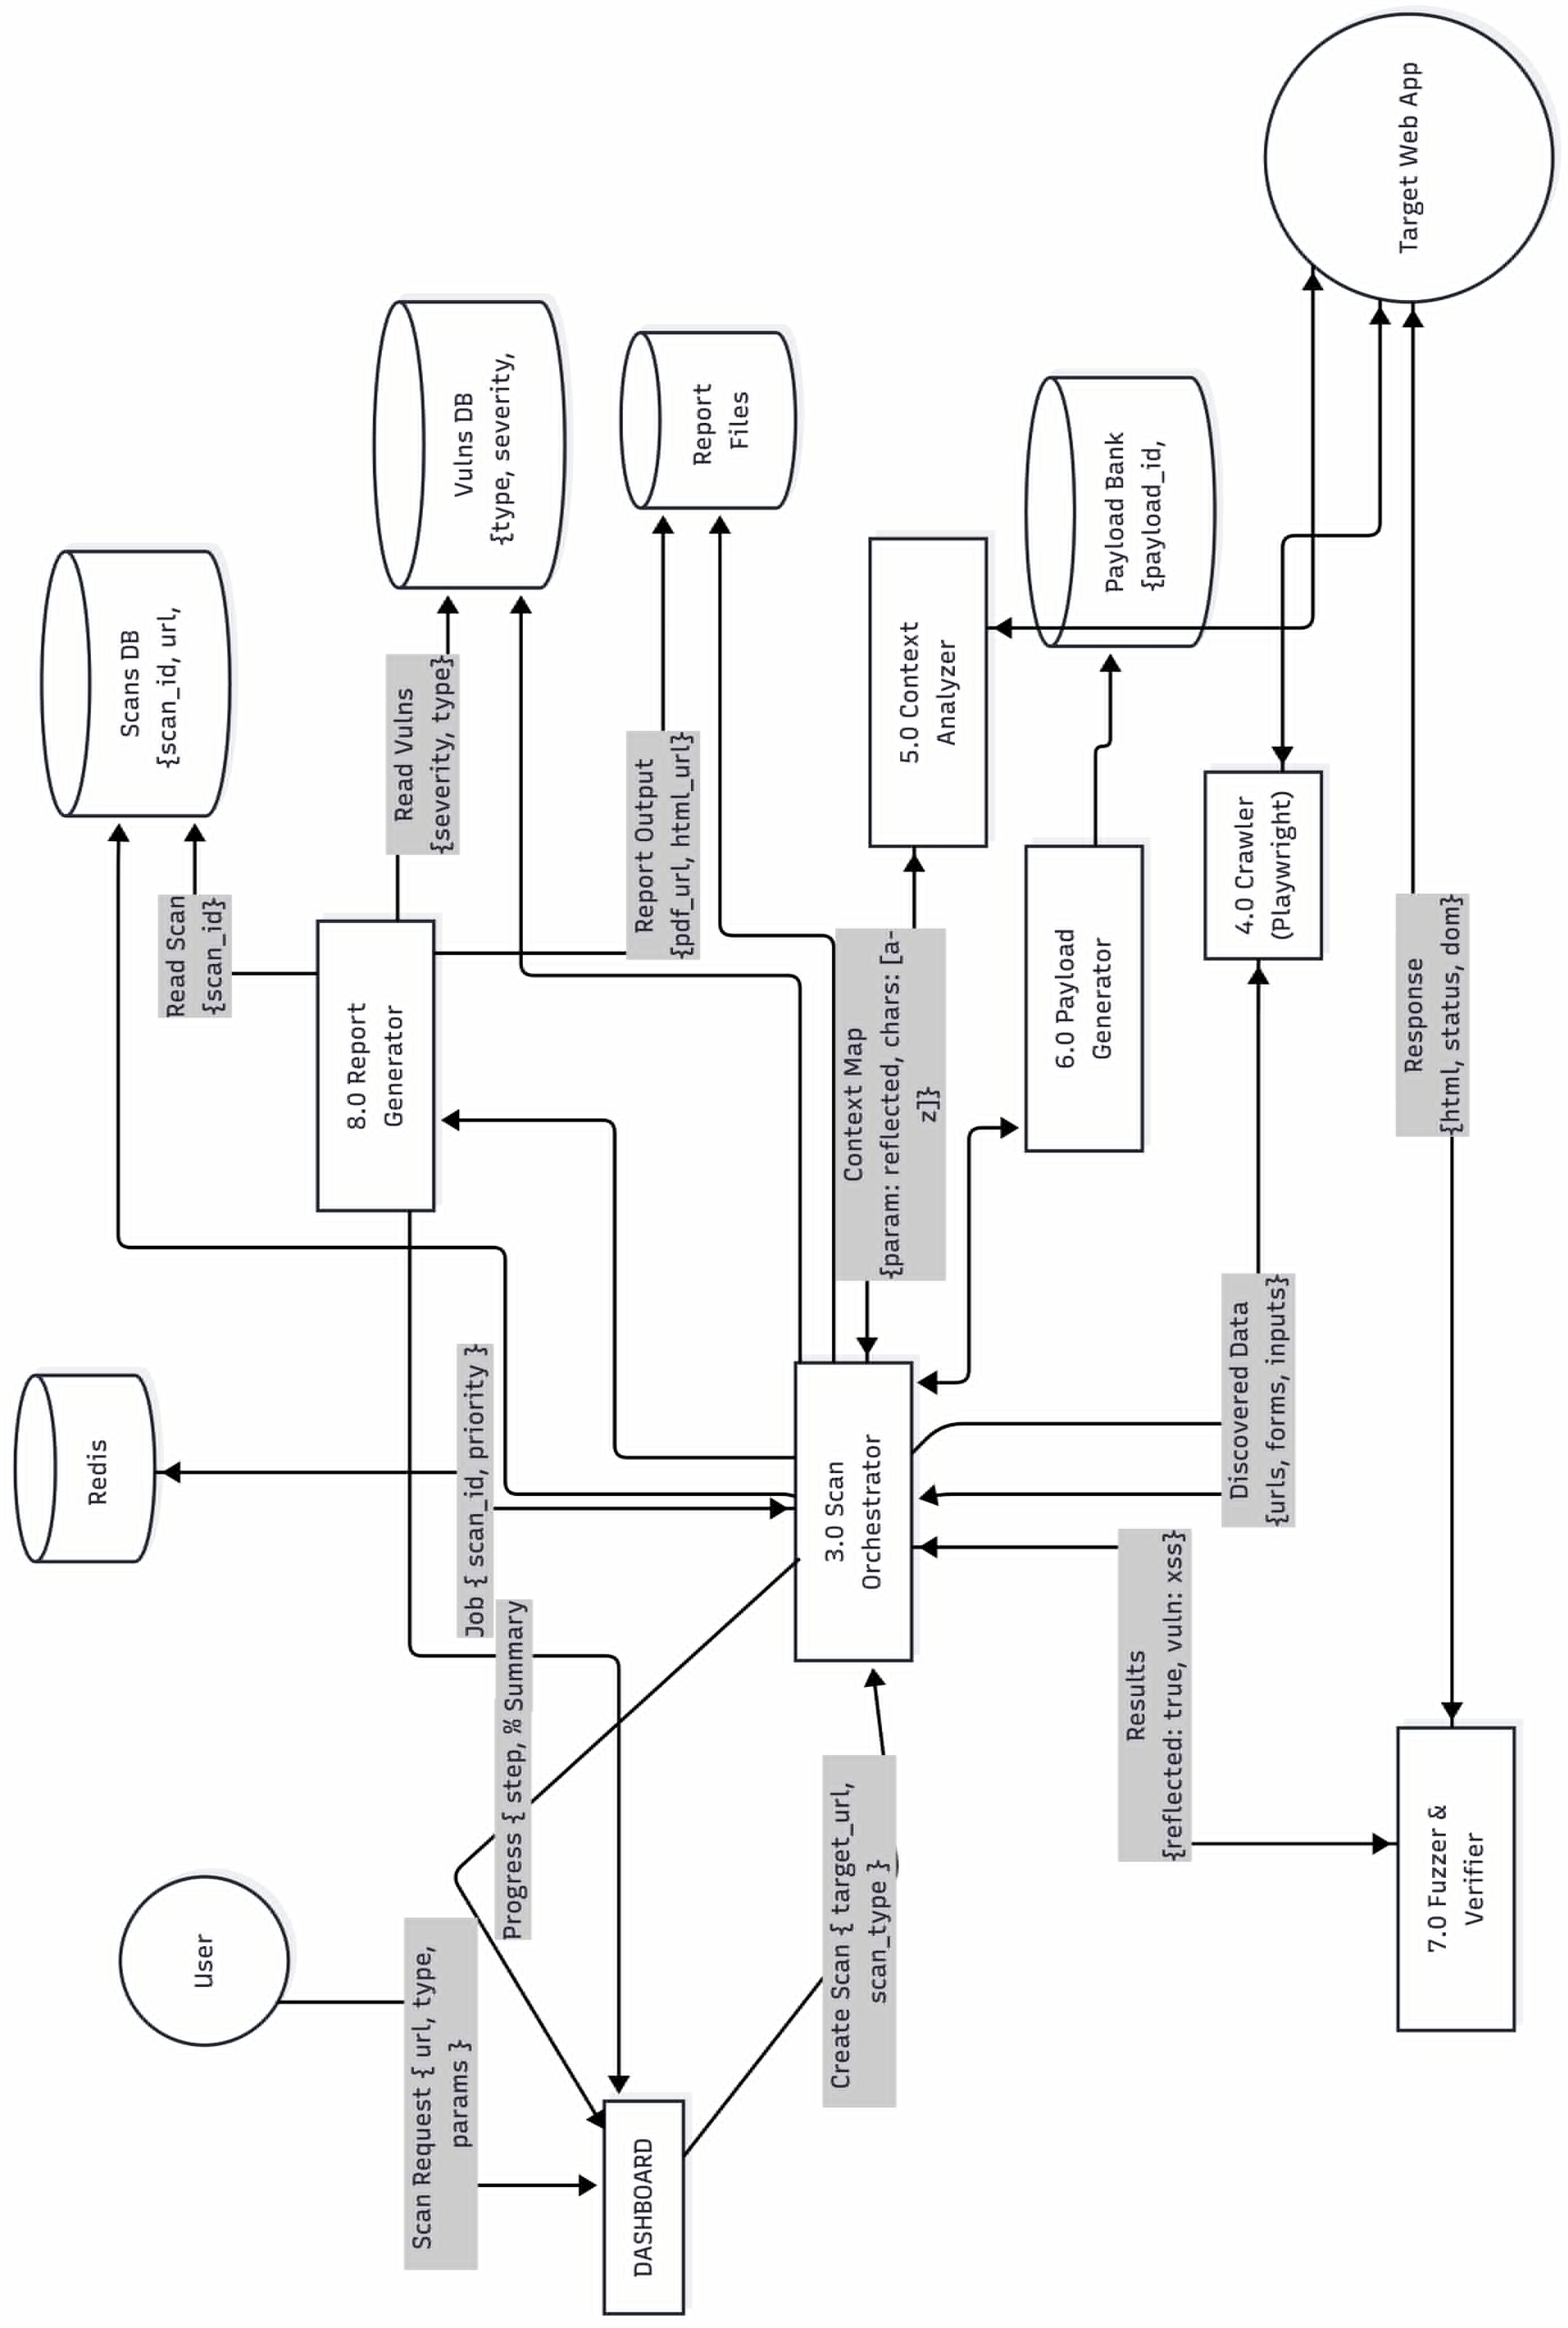
\includegraphics[angle=-90,width=1\textwidth]{figures/dfd1.jpg}
  \caption{Detailed System Architecture and Data Flow of the RedSentinel AI-Assisted XSS Scanning Framework}
  \label{fig:example_image}  
\end{figure}

\newpage
\subsection{Tech stack}
    \renewcommand{\arraystretch}{1.5}


\begin{table}[H]
    \centering
    \begin{tabular}{|p{2.7cm}|p{3cm}|p{8cm}|}
    \hline
    \textbf{Layer} &
    \textbf{Technology} &
    \textbf{Rationale} \\
    \hline
    
    Core API &
    NestJS (TypeScript) &
    Dependency injection, modular architecture, built-in validation, Swagger generation, first-class WebSocket support \\
    \hline
    
    Job Queue &
    BullMQ + Redis &
    Reliable job delivery with at-least-once semantics, priority queues, job cancellation, delayed retries, dashboard monitoring \\
    \hline
    
    AI / Security Modules &
    Python 3.11 + FastAPI &
    PyTorch/HuggingFace ecosystem for transformer models; Playwright for headless browser; Pydantic for schema validation \\
    \hline
    
    AI Model &
    DistilBERT (HuggingFace) &
    97\% of BERT accuracy at 40\% fewer parameters; fast inference suitable for scan pipeline latency requirements \\
    \hline
    
    Frontend &
    Next.js 16 + Tailwind CSS 4 &
    Server components for initial render; Socket.io client for real-time updates; Tailwind for utility-first styling \\
    \hline
    
    Database &
    PostgreSQL 16 &
    ACID compliance; jsonb columns for flexible vulnerability metadata; reliable with read-heavy workloads \\
    \hline
    
    Report Generation &
    Handlebars + Puppeteer &
    Handlebars templates for structured HTML reports; Puppeteer renders HTML to high-fidelity PDF \\
    \hline
    
    Containerization &
    Docker Compose &
    Service isolation; deterministic builds; health-check-based startup ordering; volume management for persistent data \\
    \hline
    \end{tabular}
    \caption{Technology Stack Rationale}
    
\end{table}
\section{Module Design and Implementation}
\subsection{NestJS Core Service}
\subsubsection{Module Section}
The NestJS core is organized into seven modules following NestJS's opinionated module system.
Each module encapsulates its own controllers, services, and test files.
   \begin{table}[H]
    \centering
    \begin{tabular}{|p{2.7cm}|p{5cm}|p{4cm}|}
    \hline
    \textbf{Module} &
    \textbf{Responsibility} &
    \textbf{Key Classes} \\
    \hline
    
    ScanModule &
    Scan CRUD operations, lifecycle management, WebSocket event emission &
    ScanController, ScanService, ScanGateway \\
    \hline
    
    QueueModule &
    BullMQ job production and consumption; pipeline orchestration &
    ScanProducer, ScanProcessor \\
    \hline
    
    ReportModule &
    HTML/PDF/JSON report generation and file management &
    ReportService, ReportController \\
    \hline
    
    ModulesBridge Module &
    HTTP client wrappers for all three Python services &
    ContextClient, PayloadGenClient, FuzzerClient \\
    \hline
    
    AuthModule &
    API key extraction and validation guard &
    ApiKeyGuard, AuthService \\
    \hline
    
    HealthModule &
    Aggregated health check endpoint polling all dependencies &
    HealthController, PythonHealthIndicator \\
    \hline
    
    CommonModule &
    Shared interfaces, exception filters, utility functions &
    GlobalExceptionFilter, ValidationPipe \\
    \hline
    \end{tabular}
    \caption{NestJS Core Module Structure}
    \end{table}
\subsubsection{Scan Module}
\subsubsection{ Scan Controller and Service}
The ScanController exposes the public REST API surface, delegating all business logic to ScanService. Controller methods are thin: they validate incoming DTOs using class-validator decorators, call ScanService, and return HTTP responses. The ScanService is responsible for:
\begin{itemize}[itemsep=2pt, topsep=-15pt]
    \item Persisting new scan records to PostgreSQL via TypeORM repositories.
    \item Enqueuing scan jobs to BullMQ via ScanProducer.
    \item Retrieving scan status and vulnerability lists for GET endpoints.
    \item Handling scan cancellation by removing the BullMQ job and updating scan status
    \item Providing paginated scan listing with sorting and filtering capabilities. 
\end{itemize}
\subsubsection{ BullMQ Queue Architecture}
BullMQ is a Redis-backed job queue library for Node.js. RedSentinel uses a single 'scan-queue' with the following configuration:
\begin{itemize}[itemsep=2pt, topsep=-15pt]
    \item Concurrency: 2 simultaneous scan jobs per worker instance (configurable). This prevents memory exhaustion from concurrent Playwright browser instances.
    \item Retry policy: Up to 3 retries with exponential backoff starting at 5 seconds. Scan jobs that fail after all retries are moved to a failed state and the scan record is updated accordingly.
    \item Job timeout: 60,000 ms default (configurable via DEFAULT\_\allowbreak TIMEOUT\_\allowbreak MS). Long-running scans against large targets require extended timeouts.
    \item Job removal: Completed jobs are removed after 24 hours. Failed jobs are retained for 7 days for post-mortem debugging.
\end{itemize}

\textbf{M/G/c Queue Model}

Scan requests arrive as a Poisson process with rate $\lambda$ (arrivals/sec). Each scan has a generally distributed service time $S$ with mean $
\mathbb{E}[S] = \frac{1}{\mu}
$
and second moment
$ \mathbb{E}[S^2].$
The system has $c$ concurrent worker processes. Under these assumptions:
\subparagraph*{Traffic Intensity per Server}

\[
\rho = \frac{\lambda}{c\mu}
\]

\subparagraph*{Stability Condition}

\[
\rho < 1
\iff
\lambda < c\mu
\]

\subparagraph*{Pollaczek--Khinchine Mean Waiting Time (M/G/1 Baseline)}

\[
W_q =
\frac{\lambda \, \mathbb{E}[S^2]}
     {2(1-\rho)}
\]

\subparagraph*{Coefficient of Variation}

\[
C_v =
\frac{\sqrt{\mathrm{Var}[S]}}
     {\mathbb{E}[S]}
\]

\subparagraph*{M/G/c Kingman Approximation}

\[
W_q \approx
\frac{C_v^2 + 1}{2}
\cdot
\frac{\rho^{\sqrt{2(c+1)} - 1}}
     {c(1-\rho)}
\cdot
\mathbb{E}[S]
\]

This gives system operators a formula to tune
\texttt{DEFAULT\_MAX\_PAYLOADS}
and concurrency $c$ to meet a target P99 scan latency SLA, without violating Redis memory pressure bounds.


\subsubsection{WebSocket Gateway}
The ScanGateway implements the Socket.io server using NestJS's @WebSocketGateway decorator. Clients subscribe to scan-specific rooms identified by scan ID. The gateway emits four
event types:

\begin{table}[h]
\centering
\renewcommand{\arraystretch}{1.5}
\begin{tabular}{|p{3cm}|p{6cm}|p{4cm}|}
\hline
\textbf{Event} &
\textbf{Payload} &
\textbf{Trigger} \\
\hline

scan:progress &
\{ scanId, phase, progress, message \} &
Each pipeline phase transition; progress percentage updates \\
\hline

scan:finding &
\{ scanId, vulnerability: VulnerabilityDto \} &
Each confirmed XSS finding during fuzzing phase \\
\hline

scan:complete &
\{ scanId, summary: ScanSummaryDto \} &
Scan pipeline completion (success) \\
\hline

scan:error &
\{ scanId, error: string \} &
Unrecoverable scan failure after retries exhausted \\
\hline

\end{tabular}
\caption{WebSocket Gateway Event Types}
\end{table}

\subparagraph*{WebSocket Progress as a Continuous-Time Markov Chain}

The 5-phase scan pipeline\\
$
\texttt{CRAWL}
\rightarrow
\texttt{CONTEXT}
\rightarrow
\texttt{PAYLOAD\mbox{-}GEN}
\rightarrow
\texttt{FUZZ}
\rightarrow
\texttt{REPORT}
$ \\
can be modeled as a Continuous-Time Markov Chain (CTMC) to derive the expected completion time and phase-conditional progress distributions.

\subparagraph*{State Space}
$
S =
\{
0=\texttt{IDLE},
1=\texttt{CRAWL},
2=\texttt{CONTEXT},
3=\texttt{PAYLOAD\mbox{-}GEN},
4=\texttt{FUZZ},
5=\texttt{REPORT},
6=\texttt{DONE}
\}
$

\subparagraph*{Generator Matrix}

Let, $ Q \in \mathbb{R}^{7 \times 7} $denote the CTMC generator matrix, defined by:

\[
Q_{ii} = -\mu_i,
\qquad
Q_{i,i+1} = \mu_i
\quad
\text{for \{} i=0,\dots,5 
\text{\}}
\quad
\text{ and } 
\quad
Q_{6j} = 0 
\]

where state \(6\) is an absorbing state corresponding to scan completion.

\subparagraph*{Expected Scan Completion Time}

The expected remaining completion time starting from phase \(i\) is:

\[
\mathbb{E}[T_{\text{total}} \mid \text{phase}=i]
=
\sum_{k=i}^{5}
\frac{1}{\mu_k}
\]

\subparagraph*{Conditional Progress Distribution}

The probability of being in phase \(k\) at time \(t\) is:

\[
p_k(t)
=
\Pr(\text{phase}=k \text{ at time } t)
=
\left[e^{Qt}\right]_{0,k}
\]

where \(e^{Qt}\) denotes the matrix exponential of the generator matrix.

The WebSocket event
\texttt{scan:progress}
broadcasts the empirical phase index \(k\) and the fraction of payloads processed within phase \(4\) (\texttt{FUZZ}), providing users with a fine-grained real-time estimate of \(p_k(t)\).

\subsubsection{Report Engine}
The ReportService uses Handlebars templates to render HTML reports from scan data, then employs Puppeteer to render the HTML to PDF. The report engine supports three output formats HTML, PDF and JSON.
\subparagraph*{Vulnerability Scoring via CVSS and Formal Risk Calculus}
The report engine assigns a severity score to each discovered XSS vulnerability. This section derives the scoring formally, grounding the CVSS v3.1 base score in a utility-theoretic risk model.
\subparagraph*{CVSS v3.1 Base Score Formula}
\subparagraph*{CVSS Base Score Computation}

CVSS assigns numeric sub-scores to the following security metrics:

\[
\text{AV},\;
\text{AC},\;
\text{PR},\;
\text{UI},\;
\text{S},\;
\text{C},\;
\text{I},\;
\text{A}
\]

where:

\begin{itemize}
    \item AV = Attack Vector
    \item AC = Attack Complexity
    \item PR = Privileges Required
    \item UI = User Interaction
    \item S = Scope
    \item C = Confidentiality Impact
    \item I = Integrity Impact
    \item A = Availability Impact
\end{itemize}

\subparagraph*{Impact Sub-score}

The Impact Sub-score Base is defined as:


$ \mathrm{ISCBase}
=
1
-
(1-\mathrm{ImpactConf})
(1-\mathrm{ImpactInteg})
(1-\mathrm{ImpactAvail})$


The final impact score is:

\[
\mathrm{ISC}
=
\begin{cases}
6.42 \cdot \mathrm{ISCBase},
& \text{if Scope = UNCHANGED}
\\[1em]
7.52(\mathrm{ISCBase}-0.029)
-
3.25(\mathrm{ISCBase}-0.02)^{15},
& \text{if Scope = CHANGED}
\end{cases}
\]

\subparagraph*{Exploitability Sub-score}

\[
\mathrm{Exploitability}
=
8.22
\cdot
\mathrm{AV}
\cdot
\mathrm{AC}
\cdot
\mathrm{PR}
\cdot
\mathrm{UI}
\]

\subparagraph*{Base Score}

\[
\mathrm{Base}
=
\begin{cases}
0,
& \text{if } \mathrm{ISC} \le 0
\\[1em]
\mathrm{Roundup}
\left(
\min(\mathrm{ISC}+\mathrm{Exploitability},\,10)
\right),
& \text{if Scope = UNCHANGED}
\\[1em]
\mathrm{Roundup}
\left(
\min(1.08(\mathrm{ISC}+\mathrm{Exploitability}),\,10)
\right),
& \text{if Scope = CHANGED}
\end{cases}
\]

where \(\mathrm{Roundup}(\cdot)\) rounds to one decimal place toward positive infinity.

\subparagraph*{Example: Reflected XSS}

For reflected XSS (the primary target of RedSentinel), the typical CVSS metric values are:


$
\mathrm{AV} : N  (0.85)\text{, } 
\mathrm{AC} : L  (0.77) \text{, }
\mathrm{PR} : N  (0.85) \text{, }
\mathrm{UI} : R  (0.62) \text{, }
\mathrm{S}  : C \text{, }
\mathrm{C}  : L  (0.22)
\text{, } \quad
\mathrm{I}  : L  (0.22)\text{, }
\mathrm{A}  : N  (0.00)\text{, }
$


yielding a Base Score of approximately: $\mathrm{Base} \approx 6.1$ corresponding to a \texttt{MEDIUM} severity classification.
\subparagraph*{Expected Loss Model}
Beyond CVSS, the report engine can expose an expected monetary loss model. Given an asset value $V_asset$, an annualised attack frequency $\lambda_a$, and the CVSS-derived probability of successful exploit $P_exploit$:

\subparagraph*{Expected Loss and Annual Loss Expectancy}

The expected loss (\(\mathrm{EL}\)) from a vulnerability can be modeled as:

\[
\mathrm{EL}
=
\lambda_a
\cdot
P_{\mathrm{exploit}}
\cdot
V_{\mathrm{asset}}
\cdot
(1-\mathrm{control}_{\mathrm{effectiveness}})
\]

where:

\begin{itemize}
    \item \(\lambda_a\) = attack arrival rate
    \item \(P_{\mathrm{exploit}}\) = probability of successful exploitation
    \item \(V_{\mathrm{asset}}\) = asset value or potential loss magnitude
    \item \(\mathrm{control}_{\mathrm{effectiveness}}\) = effectiveness of deployed security controls
\end{itemize}

\subparagraph*{Exploit Probability Approximation}

The exploit probability is approximated from the CVSS exploitability score:

\[
P_{\mathrm{exploit}}
\approx
\frac{\mathrm{Exploitability}}{10}
\]

which normalizes the CVSS exploitability metric into the range \([0,1]\).

\subparagraph*{Annual Loss Expectancy (ALE)}

The Annual Loss Expectancy is defined as:

\[
\mathrm{ALE}
=
\frac{
\mathrm{EL} \cdot 365
}{
\mathrm{MTTR}
}
\qquad
\text{
where, 
 $\mathrm{MTTR}$ = Mean Time To Remediate (days)}
 \]

\subparagraph*{Risk Reduction from Patching}

The reduction in annualized risk after remediation is:

\[
\Delta \mathrm{ALE}
=
\mathrm{ALE}_{\mathrm{before}}
-
\mathrm{ALE}_{\mathrm{after}}
\]

Assuming successful patching eliminates exploitability,  $ P_{\mathrm{exploit}} \to 0 $ then: $\mathrm{ALE}_{\mathrm{after}} \to 0$ 
 
\[ \therefore \Delta \mathrm{ALE} = \mathrm{ALE}_{\mathrm{before}}\]

meaning the full expected annualized loss associated with the vulnerability is removed after remediation.
\subsection{ Context Module (Python :5001)}

The Context module is responsible for the second phase of the scan pipeline: analyzing each injection point discovered by the crawler to determine the XSS injection context. This is the AI intensive component of the system.
\subsubsection{API Contract}
The module exposes a FastAPI application with the following primary endpoints:
\begin{table}[h]
\centering
\renewcommand{\arraystretch}{1.2}
\begin{tabularx}{\textwidth}{|>{\raggedright\arraybackslash}p{2cm}|>{\raggedright\arraybackslash}p{5.5cm}|X|}
\hline
\textbf{Method} & \textbf{Endpoint} & \textbf{Behavior} \\
\hline

POST & \texttt{/scan} & Create a scan, enqueue it, and return the scan record \\
\hline

GET & \texttt{/scan/:id} & Return scan status and persisted vulnerabilities \\
\hline

GET & \texttt{/scans?page=\&limit=} & Return paginated scan records \\
\hline

GET & \texttt{/scan/:id/audit} & Return scan audit logs \\
\hline

GET & \texttt{/scan/:id/report} & Return \texttt{\{ reportUrl: "/reports/<id>.html" \}}; this is a pointer only \\
\hline

DELETE & \texttt{/scan/:id} & Cancel an active scan \\
\hline

DELETE & \texttt{/scans/:id} & Permanently delete one scan and its results \\
\hline

DELETE & \texttt{/scans} & Delete all scans, results, and reports \\
\hline

GET & \texttt{/reports/:scanId} & List available generated report formats and download links \\
\hline

GET & \texttt{/reports/:scanId/ ?format=html|json|pdf} & Download an existing report file \\
\hline

GET & \texttt{/reports/:scanId/ ?formats=html,json,pdf} & Regenerate selected report formats \\
\hline

GET & \texttt{/health} & Return aggregate health status \\
\hline

\end{tabularx}
\caption{Core Scan and Report API Routes}
\label{tab:scan-report-routes}
\end{table}


\subsubsection{Reflection Analysis}
Before invoking the AI classifier, the Context module performs HTTP-level reflection analysis. For each injection point, a set of probe strings are injected: a unique random alphanumeric string, an HTML tag probe (<xss-probe>), and a JavaScript probe ('<script>). The HTTP response is analyzed to determine:
\begin{itemize}
    \item Whether the probe string appears in the response body (reflection detection).
    \item The surrounding HTML context of the reflected string (parsed using BeautifulSoup).
    \item Whether the probe appears inside an HTML attribute, a JavaScript string, a URL parameter, or raw HTML content.
    \item Whether the angle brackets in the HTML tag probe were HTML-encoded (indicating server-side sanitization).
\end{itemize}
This reflection data is then combined with the page HTML to construct the input to the DistilBERT classifier.


\subsubsection{AI Context Classification}

The core of the Context module is a fine-tuned DistilBERT model that classifies injection contexts into one of eight classes: tag\_\allowbreak injection, attribute\_\allowbreak escape, event\_\allowbreak handler,dom\_\allowbreak sink,script\_\allowbreak injection, js\_\allowbreak uri,template\_\allowbreak injection and generic. The classification input is a concatenation of the probe's surrounding HTML context (up to 512 tokens) with a special [SEP] token separating the probe position marker.

The model produces a probability distribution over the eight classes. The argmax class is taken as the prediction, and the softmax probability of the winning class is reported as confidence. Points with confidence below a threshold (default 0.7) are flagged for conservative payload selection.

\subsection{Payload Generation Module (Python :5002)}

The Payload-Gen module translates context classifications into an ordered list of candidate payloads for each injection point. It combines dataset-driven selection, algorithmic mutation, obfuscation, and AI-assisted ranking.

\subsubsection{XSS Payload Dataset}

The dataset contains 59,122 labeled XSS payloads, curated from public XSS payload lists (XSSHunter, PayloadsAllTheThings, OWASP), competition writeups, and synthetically generated variants. Each payload is labeled with:

\begin{itemize}
    \item Primary context suitability (one of the eight context classes).
    \item WAF evasion technique category (none, encoding, case, comment, unicode, polyglot). 
    \item Complexity score (1-5, correlating with ability to evade filters).
    \item Verified execution flag (whether the payload has been verified to execute in a browser).
\end{itemize}

The dataset is stored as Parquet files split into train (80\%), validation (10\%), and test (10\%) splits.The splits are loaded at module startup into an in-memory Pandas Data Frame indexed by context class and complexity tier for efficient filtering.

\subsubsection{Payload Selection Algorithm}

Given a classified injection point with context C and WAF evasion flag W, the selection algorithm proceeds as follows:

\begin{enumerate}
    \item  Filter dataset to payloads with primary\_\allowbreak context == C.
    \item  If W is true, further filter to payloads with waf\_\allowbreak evasion != 'none'.
    \item Apply complexity budget: select a weighted sample favoring mid-complexity (3-4) payloads to balance evasion capability with false-positive risk.
    \item Limit initial candidate set to min(200, total filtered) payloads.
    \item  Submit candidates to ranker model for scoring and ranking
    \item Return top-N payloads (default N = DEFAULT\_\allowbreak MAX\_\allowbreak PAYLOADS = 50).
\end{enumerate}

These deterministic rules form the foundation for supervised ML labels and validation.

\subsubsection{Mutation Engine}

The mutation engine applies transformations to selected payloads to increase diversity and evade signature-based filters. Eight mutation strategies are implemented:


\begin{enumerate}
    \item HTML entity encoding: Replace characters with their HTML entity equivalents (e.g., $<$becomes \&lt; or \&\#60;).

    \item URL encoding: Percent-encode characters (e.g., $<$ becomes \%3C). Double and triple encoding variants are also available.
    \item Unicode escaping: Replace characters with Unicode escape sequences within JavaScript contexts (e.g., \textbackslash u003c for $<$).
    \item Comment injection: Insert HTML or JavaScript comment strings within keywords to break signature matching (e.g., $<sc<!--x-->ript>$).
    \item Whitespace manipulation: Insert tab characters, non-breaking spaces, or line breaks between tokens.
    \item Attribute quoting: Vary quote styles around attribute values (single, double, backtick, no quote).
    \item Event handler substitution: Replace common event handlers (\texttt{onerror, onload}) with lesscommon but functional equivalents (\texttt{onfocus, onmouseover, onanimationend}).

\end{enumerate}
\subsubsection{Probabilistic Context-Free Grammar}
A probabilistic context-free grammar (PCFG) is defined as$
G = (V, \Sigma, R, S, P)$
where \(V\) is the set of non-terminal symbols, \(\Sigma\) is the set of terminal symbols
(e.g., HTML/JavaScript tokens), \(R\) is the set of production rules, \(S\) is the start symbol,
and $ P : R \rightarrow (0,1]$ is a probability function assigning probabilities to production rules such that, for every \(A \in V\),

\[
\sum_{A \rightarrow \alpha \in R} P(A \rightarrow \alpha) = 1
\]

The probability of a complete derivation tree \(\tau\) is given by

\[
P(\tau) =
\prod_{(A \rightarrow \alpha) \in \tau}
P(A \rightarrow \alpha)
\]

The marginal probability of a payload string \(w\) is

\[
P(w) =
\sum_{\tau \,:\, \mathrm{yield}(\tau)=w}
P(\tau)
\]

Mutation is modeled as a stochastic rewrite system. A payload
\(p \in \Sigma^{*}\) is transformed by a mutation operator
\(M_{\theta}\) drawn from a parameterized family:

\[
p' \sim M_{\theta}(p)
\]

where,
$
M_{\theta}$ =
\{ 
\texttt{case\_fold},\allowbreak
\texttt{entity\_encode},\allowbreak
\texttt{unicode\_escape},\allowbreak
\texttt{ js\_comment} \linebreak \texttt{\_insert},\allowbreak
\texttt{event\_handler\_substitute},\allowbreak
\ldots
\}


The conditional probability of generating \(p'\) from \(p\) under parameters
\(\theta\) is

\[
P(p' \mid p, \theta)
=
\prod_{i}
P(m_i \mid \mathrm{context}_i, \theta)
\]

\subsubsection{ Payload Ranking}
A secondary lightweight gradient-boosted classifier (XGBoost) trained on historical scan data ranks the mutated payload candidates by estimated probability of successful execution against the specific target. Features used for ranking include payload length, encoding complexity, context match score, WAF evasion technique, and historical success rate from the training dataset. The ranker outputs a score in [0,1] for each payload, which is used to sort the final list before returning to the Core.
\subsubsection{Payload Ranking via Expected Bypass Probability}
The fuzzer ranks each candidate payload \(p_j\) according to its estimated probability of
bypassing WAF filtering. Given an observation model \(O\) that assigns a bypass probability
\(b(p,w)\) for a WAF signature set \(w\), the ranking score is defined as

\[
\mathrm{score}(p_j)
=
\mathbb{E}_{w}\!\left[b(p_j,w)\right]
\cdot
\mathbb{E}_{\mathrm{ctx}}
\!\left[
P(\mathrm{reflect}\mid \mathrm{ctx}, p_j)
\right]
\]

Expanding the expectation over WAF signatures yields

\[
\mathrm{score}(p_j)
=
\left(
\sum_{w}
b(p_j,w)\,\pi(w)
\right)
\cdot
P(\mathrm{reflect}\mid \mathrm{ctx}, p_j)
\]

where $\pi(w)$ denotes the prior probability distribution over observed WAF signatures, and $P(\mathrm{reflect}\mid \mathrm{ctx}, p_j)$ represents the context-conditioned reflection probability produced by the sigmoid head of the context analysis module.

Payloads are emitted in descending order of
\(\mathrm{score}(p_j)\), ensuring that the most contextually appropriate and WAF-evasive
payloads are fuzzed first, thereby reducing the total number of requests required during
testing.
\subsection{Payload Diversity}
Selecting only the highest-ranked payloads risks converging to a narrow mode of the payload distribution, missing novel bypass vectors. Information theory provides the right objective to maximise coverage entropy subject to a budget constraint.
\subsubsection{Maximum Entropy Payload Sampling}

\subparagraph*{Entropy-Regularised Payload Selection}

Let
$q = (q_1, \dots, q_n) $be a probability distribution over the \(n\) candidate payloads in the payload bank.

\subparagraph*{Shannon Entropy}

The Shannon entropy of the selection distribution is:

\[
H(q)
=
-
\sum_{j=1}^{n}
q_j \log q_j
\]

\subparagraph*{Constrained Optimisation Problem}

The objective is to select payloads that maximize expected bypass effectiveness while preserving diversity:

\[
\max_{q}
\;
\alpha
\sum_{j}
q_j \, \mathrm{score}(p_j)
+
(1-\alpha)\, H(q)
\]

subject to:

\[
\sum_{j} q_j = 1 \text{,}
\quad
q_j \ge 0 \text{,}
\quad
\sum_{j}
q_j \, \mathrm{cost}(p_j)
\le
\texttt{DEFAULT\_MAX\_PAYLOADS}
\]

where:

\begin{itemize}
    \item \(\mathrm{score}(p_j)\) denotes the effectiveness score of payload \(p_j\),
    \item \(\mathrm{cost}(p_j)\) denotes the execution cost of payload \(p_j\),
    \item \(\alpha \in [0,1]\) is the exploration--exploitation trade-off hyperparameter.
\end{itemize}

\subparagraph*{Optimal Solution}

Using Lagrange multipliers, the optimal distribution is:

\[
q_j^{*}
=
\frac{
\exp\!\left(
\frac{
\alpha \, \mathrm{score}(p_j)
}{
1-\alpha
}
\right)
}{
\sum_{k}
\exp\!\left(
\frac{
\alpha \, \mathrm{score}(p_k)
}{
1-\alpha
}
\right)
}
\]

This is a Gibbs (Boltzmann) distribution with temperature

\[
T = \frac{1-\alpha}{\alpha}
\]

\subparagraph*{Limiting Behaviour}

As $\alpha \to 1$\text{, } $ q^{*}\to\arg\max \mathrm{score}(p_j) $ recovering the greedy ranking strategy.

While as $\alpha \to 0$\text{, } $ q^{*} \to \text{Uniform}(1,\dots,n) $ resulting in approximately uniform sampling over the full \(59,122\) payload bank.

The default setting $ \texttt{DEFAULT\_MAX\_PAYLOADS} = 50$ implicitly fixes a computational budget. Tuning \(\alpha\) controls the exploration--exploitation trade-off without changing the overall payload budget.






\subsection{Fuzzer Module (Python :5003)}
The Fuzzer module executes the actual injection phase: sending HTTP requests with payloads,analyzing responses for reflection, and verifying suspected vulnerabilities using a headless browser. It is the most resource-intensive module due to Playwright browser automation.

\subsubsection{HTTP injection}
The Fuzzer accepts a list of injection targets with associated ranked payload lists. For each (target,
payload) pair:
\begin{enumerate}
    \item Construct the HTTP request with the payload substituted for the injection parameter value.
    \item Send the request using httpx (async HTTP client) with configurable timeout and UserAgent.
    \item Analyze the HTTP response body for payload reflection using string matching and lightweight HTML parsing.
    \item If reflection is detected, record the injection point, payload, and reflection context for browser verification.
\end{enumerate}
The injection loop is parallelized using asyncio task groups with a configurable concurrency limit (default 10 simultaneous requests) to avoid overwhelming the target or triggering rate limiting.
\subsubsection{ Headless Browser Verification}
Raw reflection detection produces false positives (e.g., the payload appears in HTML but is encoded and will not execute). The Fuzzer performs browser verification for each candidate finding:
\begin{enumerate}
    \item Launch a Playwright Chromium instance in headless mode with JavaScript enabled.
    \item Navigate to the URL with the injected payload in the target parameter.
    \item  Inject a JavaScript listener for the verification event (typically window.onerror or a custom event triggered by the payload).
    \item Wait for JavaScript execution or timeout (5 seconds default).
    \item If the JavaScript listener fires, the vulnerability is confirmed; record as CONFIRMED with severity HIGH.
    \item If navigation completes without JavaScript execution, downgrade to SUSPECTED with severity MEDIUM.
\end{enumerate}

\subsubsection{DOM Sink Analysis}
Beyond URL parameter injection, the Fuzzer also performs DOM sink analysis to detect DOMbased XSS:

\begin{itemize}
    \item Use Playwright to navigate the target page and extract all JavaScript source files.
    \item Apply static analysis to identify calls to known dangerous sinks: innerHTML, outerHTML, document.write, eval, setTimeout/setInterval with string arguments, location.href assignments.
    \item Trace data flow from attacker-controlled sources (location.hash, location.search, document.URL, document.referrer, window.name) to identified sinks.
    \item For identified source-to-sink flows, generate a taint-based proof-of-concept URL and verify in browser.
\end{itemize}
\subsubsection{Training Data Collection}
The Fuzzer module implements a passive learning loop: successful and failed injection attempts are serialized to a training\_\allowbreak data volume as JSONL files. This data can be used to periodically retrain the payload ranker model, progressively improving ranking accuracy for specific target types over time.

\subsection{AI Model Design and Training}
\subsubsection{DistilBERT for Context Classification}
DistilBERT (Distilled BERT) is a transformer-based language model introduced by Sanh et al.(2019) at Hugging Face\cite{sanh2019distilbert}. It is produced by knowledge distillation from BERT-base, reducing the number of transformer layers from 12 to 6 while retaining 97\% of BERT's performance on the GLUEbenchmark. The model has approximately 66 million parameters.

For the context classification task, DistilBERT's pre-trained weights are loaded from the 'distilbertbase-uncased' checkpoint. A classification head is appended to the [CLS] token embedding: a linear layer projecting from the 768-dimensional hidden state to 6 output logits (one per context class), followed by softmax normalization.

\begin{figure}[H]
    \centering
    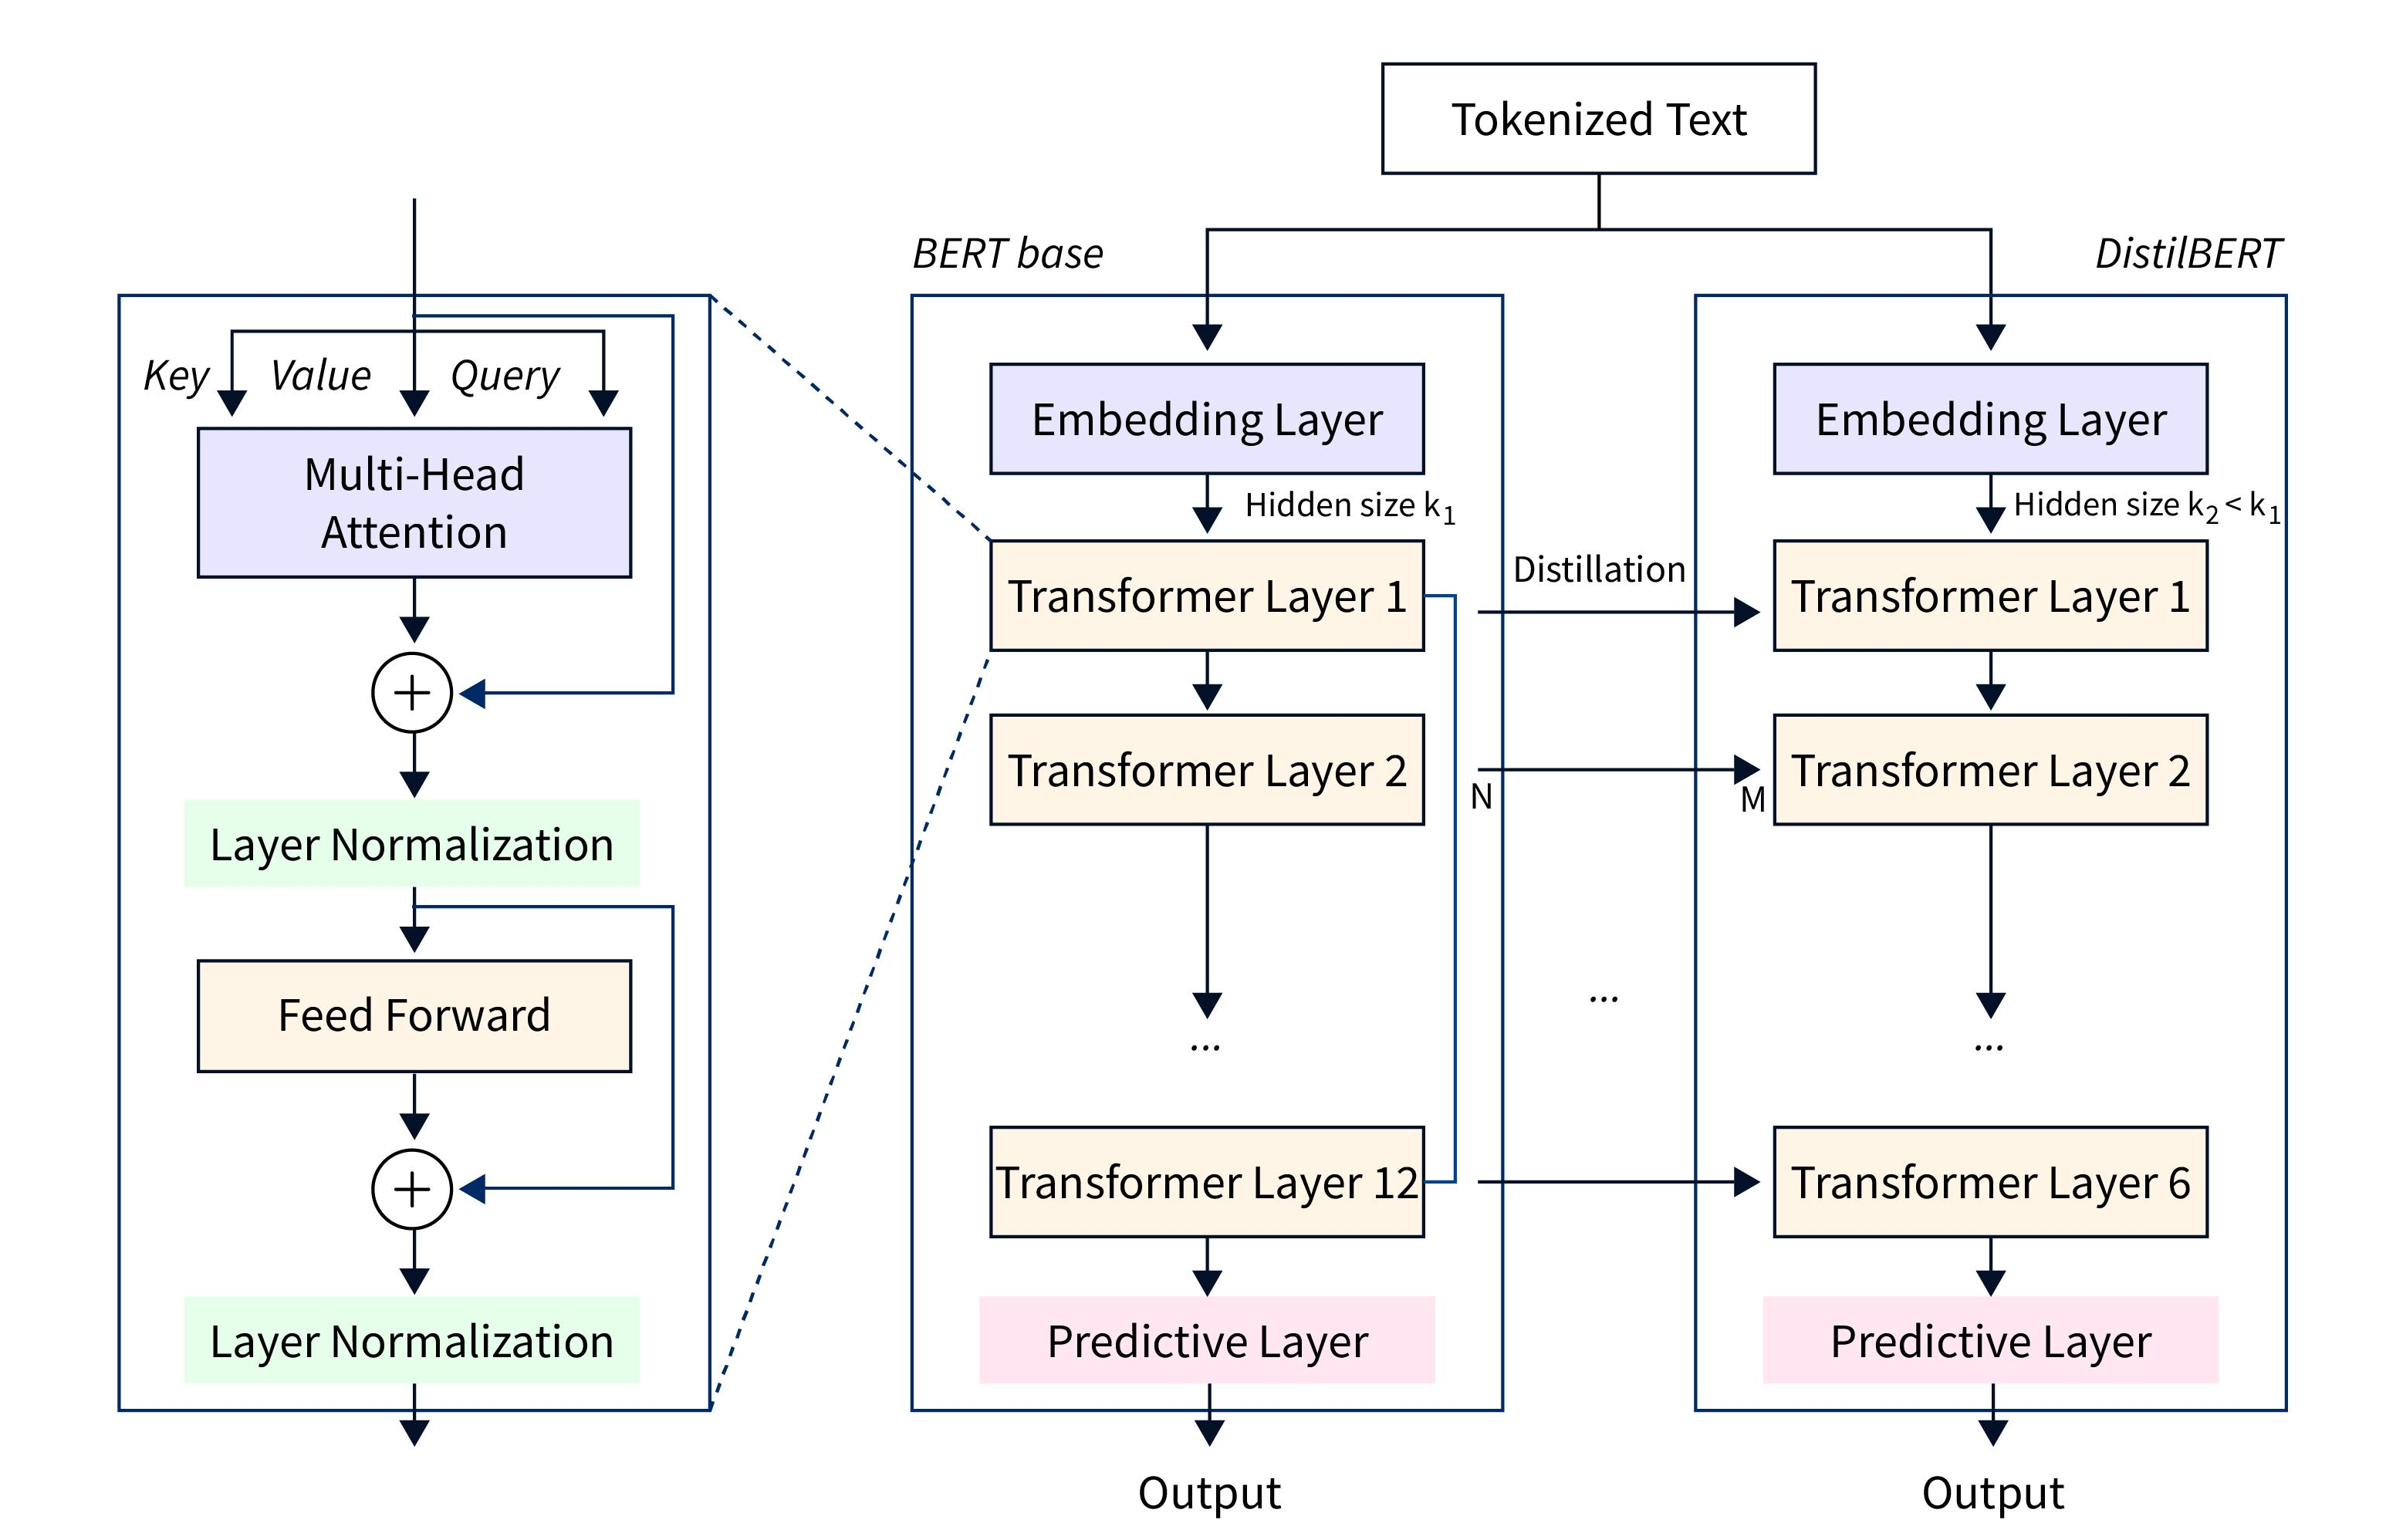
\includegraphics[width=1\linewidth]{figures/distilbert_architecture.png}
    \caption{Distilbert Architecture}
    \label{fig:distilbert_architecture}
\end{figure}

\subsubsection{Input Representation}
The input to the classifier is a tokenized string of the form:
\begin{Verbatim}[fontsize=\footnotesize]
[CLS] <surrounding HTML context> [SEP] <injection position marker> [SEP]
\end{Verbatim}
The surrounding HTML context is extracted from the page HTML around the injection point using BeautifulSoup: the 100 characters before and 100 characters after the injected probe string are taken, limited to the containing HTML element. The injection position marker is a description string generated from the reflection analysis (e.g., 'inside attribute value double-quoted' or 'inside script block string literal'). The combined input is truncated to 512 tokens using the DistilBERT tokenizer with WordPiece tokenization. Padding is applied to a fixed sequence length of 256 tokens for batch training efficiency.

\subsubsection{Training Methodology}
The classifier is fine-tuned on the labeled context classification dataset using the following training configuration:

\begin{table}[h]
    \centering
    \begin{tabular}{|p{2.7cm}|p{4cm}|p{7.3cm}|}
      \hline
        Hyperparameter & Value  &Rationale \\
         \hline
        Optimizer &AdamW  & Weight decay regularization; standard for transformer fine-tuning\\ \hline
         Learning rate&2e-5  &Recommended range for BERT-family models; prevents catastrophic forgetting
 \\ \hline
         LR scheduler&Linear warmup + cosine decay  & 5\% warmup steps; prevents early training instability\\ \hline
         
         Batch size & 32 (gradient accumulated) &Effective batch of 32; balances memory and gradient noise \\ \hline
         
         Epochs &10 with early stopping (patience 3)  & Prevent overfitting; restore best checkpoint\\ \hline
         Loss function & Cross-entropy &Prevent overfitting; restore best checkpoint \\ \hline
         Dropout &0.1 (inherited from DistilBERT)  & Regularization in attention and FFN layers\\ \hline
         Max\textcolor{white}{\_\allowbreak }sequence length& 256 tokens & Covers majority of injection contexts without padding overhead
\\
    \hline
    \end{tabular}
    \caption{DistilBERT Fine-Tuning Hyperparameters}
    
\end{table}

\subsubsection{Training Dataset}
The context classification dataset was constructed from three sources: 
\begin{enumerate}
    \item manually labeled injection contexts from a purpose-built testbed of vulnerable web applications
    \item synthetic examples generated by inserting probe strings into HTML scraped from the Common Crawl dataset
    \item examples from public XSS challenge write-ups where the injection context is described. The final dataset contains approximately 18,000 labeled examples distributed across eight classes, with balanced sampling to mitigate class imbalance.
\end{enumerate}

\subsubsection{Model Evaluation}

The model is evaluated on a held-out test split using accuracy, per-class precision, recall, and F1- score. The confusion matrix reveals the model's primary failure mode: confusion between semantically similar contexts. In practice, this confusion has minimal impact on scanner effectiveness because payloads suitable for quoted attribute contexts are a superset of those suitable for unquoted contexts.

\subsection{API design and Contract}

\subsubsection{REST API Specification}
\textbf{Authentication}\\
All API endpoints (except /health) require authentication via the x-api-key HTTP header or the Authorization: Bearer <key> header. The API key is compared using timing-safe comparison (crypto.timingSafeEqual) against the SHA-256 hash of API\_\allowbreak KEY\_\allowbreak SECRET stored in environment configuration. If API\_\allowbreak KEY\_\allowbreak SECRET is unset, the API operates in open/development mode with all authentication bypassed.

\textbf{Endpoint Specifications:} 
\lstset{
    basicstyle=\ttfamily\scriptsize,
    frame=single,
    breaklines=true,
    columns=fullflexible,
    keepspaces=true
}

\begin{lstlisting}[language=JavaScript, showstringspaces=false]
POST /scan -- Create and Enqueue a New Scan

Request Body:
{
  {
  "url": "https://target.example",
  "options": {
    "depth": 3,
    "maxParams": 100,
    "verifyExecution": true,
    "wafBypass": true,
    "maxPayloadsPerParam": 50,
    "timeout": 60000,
    "reportFormat": "\"["html", "json"],
    "singlePage": false,
    "auth": {
      "enabled": true,
      "loginUrl": "https://target.example/login",
      "username": "alice",
      "password": "secret",
      "usernameSelector": "input"\"[name=\\"username\\"]",
      "passwordSelector": "input"\"[name=\\"password\\"]",
      "submitSelector": "button"\"[type=\\"submit\\"]",
      "postLoginWaitMs": 3000,
      "successUrlContains": "/dashboard"
    }
  }
}
}

Response 201 Created:
{
  "scanId": "uuid-v4",
  "status": "QUEUED",
  "createdAt": "2026-05-01T12:00:00Z"
}
\end{lstlisting}

\begin{lstlisting}[language=JavaScript, showstringspaces=false]
GET /scan/:id -- Retrieve Scan Status and Results
Response 200:
{
  "id": "uuid",
  "targetUrl": "https://example.com",
  "status": "RUNNING",
  "phase": "FUZZ",
  "progress": 67,
  "vulnerabilities": [{
    "id": "vuln-uuid",
    "url": "https://example.com/search?q=",
    "parameter": "q",
    "payload": "<img src=x onerror=alert(1)>",
    "context": "HTML_BODY",
    "severity": "HIGH",
    "confidence": "CONFIRMED",
     \end{lstlisting}
      \begin{lstlisting}[language=JavaScript, showstringspaces=false]
    "cvssScore": 6.1
  }],
  "stats": {
    "urlsDiscovered": 45,
    "parametersScanned": 23,
    "payloadsSent": 412,
    "vulnerabilitiesFound": 3
  }
}
\end{lstlisting}

\textbf{WebSocket Protocol}
\\
The WebSocket server uses Socket.io with the default path '/socket.io'. Clients authenticate by passing the API key as a query parameter: $ws://host:3000/socket.io?apiKey=<key>$. After connection, clients join a scan-specific room by emitting join-scan with the scan ID:
\begin{lstlisting}[language=JavaScript, showstringspaces=false]
// Client join
socket.emit('join-scan', { scanId: 'uuid' });
// Server confirmation
socket.on('joined', ({ scanId }) => { ... });
// Progress update
socket.on('scan:progress', ({
 scanId, phase, progress, message
}) => { ... });
// Real-time finding
socket.on('scan:finding', ({
 scanId, vulnerability
}) => { ... });
\end{lstlisting}
\subsubsection{Python Service API Contracts}
\textbf{Context Module (/analyze)}

The Context Module is a FastAPI service running on port 5001. It exposes `POST /analyze` and `GET /health`.The implemented request model is:

\begin{lstlisting}[language=JavaScript]
{
  "url": "https://target.example/search?q=test",
  "params": \["q"],
  "waf": "none"
\end{lstlisting}
The implemented response is a parameter map:
\begin{lstlisting}[language=JavaScript]
{
  "q": {
    "reflects\_in": "html\_body",
    "allowed\_chars": \["<", ">", "\\""],
    "context\_confidence": 0.94
  }
}
\end{lstlisting}
The module injects markers into parameters, checks whether markers are reflected, determines context using regex, DOM parsing, and AI classification when available, and fuzzes allowed special characters. When the classifier artifact is unavailable, the service must not be described as fully DistilBERT-backed; it exposes `ai\_model\_loaded` through `/health`.

\textbf{Payload-Gen Module (/generate)}\\
The Payload-Gen module accepts classified injection points with context and WAF evasion flags, and returns a sorted list of payload objects. Each payload object includes the payload string, its context suitability, mutation type applied, and estimated success score from the ranker model.
\\ \\
\textbf{Fuzzer Module (/fuzz)}
The Fuzzer/Fuzzification module accepts injection targets with payload lists and scan options (timeout, concurrency). It returns a list of finding objects, each containing the injection details, HTTP evidence, browser verification result, and severity classification.

\chapter{Deployment and Infrastructure}

\section{Docker Compose Architecture}
RedSentinel's production deployment is defined entirely in docker-compose.yml, which specifies seven services with explicit dependency ordering via health checks. This section describes each service's container configuration.
\subsection{Infrastructure Services}
Redis (redis:7-alpine) serves as the BullMQ backing store and is the first service started. It requires no persistent volume as job state is ephemeral. A health check using redis-cli ping verifies availability with 5 retries at 10-second intervals. PostgreSQL (postgres:16-alpine) stores all persistent application data. The database is initialized with a custom init.sql script that creates tables with proper constraints, indexes, and extension requirements. Data is persisted to the pgdata named volume. Health check uses pg\_\allowbreak isready.
\subsection{Python Microservice Containers}
Each Python service is built from a dedicated Dockerfile within the modules/ directory. Common to all three:
\begin{itemize}[itemsep=2pt, topsep=-15pt]
    \item Base image: python:3.11-slim for minimal attack surface.
    \item Dependencies installed from requirements.txt with no-cache-dir to minimize image size.
    \item Uvicorn ASGI server as the process runner.
    \item Non-root user execution for security.
\end{itemize}
The Context service additionally mounts the model/ directory as a read-only volume, allowing model updates without container rebuilds. The Payload-Gen service mounts dataset/splits read-only for payload database access. The Fuzzer service mounts the training\_\allowbreak data volume for persistent training data collection.
\subsection{NestJS Core Container}
The Core container is built from core/Dockerfile using a multi-stage build: a build stage compiles TypeScript to JavaScript using the NestJS CLI, and a production stage copies only the compiled output and node\_\allowbreak modules. Puppeteer requires Chromium, which is installed via Alpine packages(chromium chromium-chromedriver). The PUPPETEER\_\allowbreak EXECUTABLE\_\allowbreak PATH environment variable points to /usr/bin/chromium-browser to override Puppeteer's default download behavior. The Core depends on all five other services via condition: service\_\allowbreak healthy, ensuring the complete environment is available before scan processing begins. Reports are persisted to the reports named volume and served via a static files endpoint.
\subsection{ Dashboard Container}
The dashboard builds as a production Next.js application. NEXT\_\allowbreak PUBLIC\_\allowbreak API\_\allowbreak URL is passed as a Docker build argument to embed the API URL at build time for server-side rendering. The WebSocket URL is derived at runtime from window.location in the browser to support reverse proxy deployments without hardcoded hostnames.
\section{Development Mode}
A docker-compose.dev.yml override file modifies the production configuration for development use:
\begin{itemize}[itemsep=2pt, topsep=-15pt]
    \item Source code directories are bind-mounted into containers, enabling hot reload.
    \item NestJS Core runs with npm run start:dev (ts-node-dev with watch mode).
    \item Python services run with uvicorn --reload.
    \item Port 9229 is exposed on the Core container for Node.js debugger attachment.
\end{itemize}

\section{Environment Configuration}
All sensitive and environment-specific settings are managed via environment variables, documented in .env.example with defaults. In production, use a high-entropy API\_\allowbreak KEY \_\allowbreak SECRET, strong random POSTGRES\_\allowbreak PASSWORD, and restrict CORS\_\allowbreak ORIGIN to the dashboard hostname rather than *. Docker Compose defaults (change-me-before-deploy, rs/rs) are for development only. DEFAULT\_\allowbreak SCAN\_\allowbreak DEPTH and DEFAULT\_\allowbreak MAX \_\allowbreak PAYLOADS should be adjusted based on target size and available compute resources.
\section{Volume Management}
Three named Docker volumes manage persistent data:
\begin{itemize}
    \item pgdata: PostgreSQL data directory. Stores all scan records, vulnerability data, and report metadata.
    \item reports: Report output directory. Stores generated HTML and PDF reports. Served by the Core via a static files endpoint.
    \item training\_\allowbreak data: Fuzzer training data. Stores JSONL files of injection attempt records for model retraining.
\end{itemize}
These volumes persist across container restarts and rebuilds. They must be backed up for production deployments. Volume data can be inspected or exported using standard Docker volume commands.
\chapter{Evaluation and Results} 
\section{Evaluation Objectives}
This chapter presents a comprehensive evaluation of \textit{RedSentinel}, an AI-augmented XSS vulnerability scanner. The evaluation covers four dimensions:
\begin{enumerate}[itemsep=2pt, topsep=-15pt]
    \item context classification accuracy using a fine-tuned DistilBERT model,
    \item payload ranking effectiveness via an XGBoost ranker benchmarked against baselines
    \item end-to-end vulnerability detection performance on real and purpose-built targets
    \item comparative analysis against established open-source scanning tools.
\end{enumerate}
\section{Experimental Setup}
Benchmarks were executed against four targets: \textit{Nexora XSS Lab}, \textit{OWASP Juice Shop}, \textit{Google XSS Game}, and \textit{PortSwigger XSS Labs}, covering 87 endpoints. All runs used mock-mode injection guards where required for safe benchmarking. Comparative tool evaluations (OWASP ZAP, Dalfox, XSStrike) were conducted on same endpoint sets to ensure a fair comparison.
 

\section{Dataset Evaluation}

 
\subsection{Context Classification Dataset} 
\begin{table}[H]
  \centering
   \small
  \rowcolors{2}{rowgray}{white}
  \begin{tabular}{lrrrr}
    \toprule
    \rowcolor{headblue}
    \textbf{Context} & \textbf{Train} & \textbf{Val} & \textbf{Test} & \textbf{Total} \\
    \midrule
    tag\_injection        & 16{,}210 (70.0\%) & 3{,}473 (15.0\%) & 3{,}474 (15.0\%) & 23{,}157 \\
    attribute\_escape     & 11{,}742 (70.0\%) & 2{,}516 (15.0\%) & 2{,}516 (15.0\%) & 16{,}774 \\
    event\_handler        &  4{,}219 (70.0\%) &    904 (15.0\%) &    904 (15.0\%) &  6{,}027 \\
    dom\_sink             &  4{,}455 (70.0\%) &    955 (15.0\%) &    955 (15.0\%) &  6{,}365 \\
    script\_injection     &  1{,}774 (70.0\%) &    380 (15.0\%) &    381 (15.0\%) &  2{,}535 \\
    js\_uri               &  1{,}629 (70.0\%) &    349 (15.0\%) &    349 (15.0\%) &  2{,}327 \\
    template\_injection   &    855 (70.0\%) &    183 (15.0\%) &    183 (15.0\%) &  1{,}221 \\
    generic               &    501 (70.0\%) &    108 (15.0\%) & 107 (15.0\%) &    716 \\
    \midrule
    \textbf{Total} & \textbf{41{,}385} & \textbf{8{,}868} & \textbf{8{,}869} & \textbf{59{,}122} \\
    \bottomrule
  \end{tabular}
 \caption{Context Classification Dataset Distribution}
  \label{tab:context_dist}
\end{table}
The context classification corpus contains \textbf{59,122} labelled samples distributed across eight injection-context classes. Table \ref{tab:context_dist} shows the 70/15/15 train/validation/test split.
 

 
\subsection{Payload Dataset}

 
The payload dataset comprises \textbf{59,122} unique payloads. Table~\ref{tab:payload_source} summarises the source split and Table~\ref{tab:payload_severity} the severity distribution.
 
\begin{table}[H]
  \centering
  \caption{Payload Dataset -- Source and Severity Distribution}
  \label{tab:payload_source}
  \begin{subtable}[t]{0.45\linewidth}
    \centering
    \rowcolors{2}{rowgray}{white}
    \begin{tabular}{lrr}
      \toprule
      \rowcolor{headblue}
      \textbf{Source} & \textbf{Count} & \textbf{\%} \\
      \midrule
      Synthetic & 40{,}624 & 68.7\% \\
      Real      & 18{,}498 & 31.3\% \\
      \midrule
      \textbf{Total} & \textbf{59{,}122} & 100\% \\
      \bottomrule
    \end{tabular}
    \caption{By source}
  \end{subtable}
  \hfill
  \begin{subtable}[t]{0.45\linewidth}
    \centering
    \rowcolors{2}{rowgray}{white}
    \begin{tabular}{lrr}
      \toprule
      \rowcolor{headblue}
      \textbf{Severity} & \textbf{Count} & \textbf{\%} \\
      \midrule
      Medium & 39{,}856 & 67.4\% \\
      Low    & 10{,}087 & 17.1\% \\
      High   &  9{,}179 & 15.5\% \\
      \midrule
      \textbf{Total} & \textbf{59{,}122} & 100\% \\
      \bottomrule
    \end{tabular}
    \caption{By severity}
    \label{tab:payload_severity}
  \end{subtable}
\end{table}
\section{AI Context Classification Results}
\label{sec:context_results}
 
\subsection{DistilBERT Per-Class Performance}
 

 
\begin{table}[H]
  \centering
 \footnotesize
  \rowcolors{2}{rowgray}{white}
  \begin{tabular}{lcccc}
    \toprule
    \rowcolor{headblue}
   \textbf{Context} & \textbf{Precision} & \textbf{Recall} & \textbf{F1-score} \\
\midrule
tag\_injection      & 0.9980 & 0.9974 & 0.9977  \\
attribute\_escape   & 0.9976 & 0.9984 & 0.9980  \\
event\_handler      & 1.0000 & 0.9923 & 0.9961 \\
dom\_sink           & 0.9927 & 0.9948 & 0.9937  \\
script\_injection   & 0.9819 & 0.9974 & 0.9896  \\
js\_uri             & 0.9886 & 0.9971 & 0.9929  \\
template\_injection & 0.9892 & 1.0000 & 0.9946  \\
generic             & 0.9604 & 0.9065 & 0.9327  \\
  \end{tabular}
   \caption{DistilBERT Context Classification -- Per-Class Metrics}
  \label{tab:distilbert_clf}
\end{table}
 A DistilBERT model was fine-tuned for HTML injection-context classification. Table~\ref{tab:distilbert_clf} reports per-class precision, recall, and F1-score on the held-out test split.
\begin{figure}[H]
  \centering
  \begin{tikzpicture}
    \begin{axis}[
      ybar,
      width=13cm, height=6.5cm,
      bar width=0.55cm,
      ylabel={F1-Score},
      ymin=0.80, ymax=1.03,
      symbolic x coords={
        script\_inj.,
        event\_hdlr,
        js\_uri,
        attr\_escape,
        tag\_inj.,
        dom\_sink,
        generic,
        tmpl\_inj.
      },
      xtick=data,
      x tick label style={rotate=30, anchor=east, font=\small},
      nodes near coords,
      nodes near coords align={vertical},
      every node near coord/.style={font=\scriptsize, /pgf/number format/.cd, fixed, precision=3},
      grid=major,
      grid style={dashed,gray!30},
      ytick={0.80,0.85,0.90,0.95,1.00},
      enlarge x limits=0.08,
    ]
      \addplot[fill=primary, draw=primary!70!black] coordinates {
        (script\_inj.,  0.989)
        (event\_hdlr,   0.992)
        (js\_uri,       0.997)
        (attr\_escape,  0.998)
        (tag\_inj.,     0.997)
        (dom\_sink,     0.993)
        (generic,       0.932)
        (tmpl\_inj.,    0.994)
      };
    \end{axis}
  \end{tikzpicture}
  \caption{DistilBERT F1-score per context class. All classes exceed 0.96 except \texttt{template\_injection} (0.875), which has limited training support (855 samples).}
  \label{fig:f1_bar}
\end{figure}

 \subsection{Confusion Matrix}
 
Table~\ref{tab:confusion} shows the confusion matrix for the test split. Rows represent true labels; columns represent predicted labels. Class order: \textit{script\_injection, event\_handler, js\_uri, tag\_injection, template\_injection, dom\_sink, attribute\_escape, generic}.
\begin{table}[H]
  \centering
  
  \setlength{\tabcolsep}{4pt}
  \begin{tabular}{l|cccccccc}
    \toprule
    \rowcolor{headblue}
    & \rotatebox{60}{\small script\_inj.}
    & \rotatebox{60}{\small event\_hdlr}
    & \rotatebox{60}{\small js\_uri}
    & \rotatebox{60}{\small tag\_inj.}
    & \rotatebox{60}{\small tmpl\_inj.}
    & \rotatebox{60}{\small dom\_sink}
    & \rotatebox{60}{\small attr\_escape}
    & \rotatebox{60}{\small generic} \\
    \midrule
    
    script\_inj. & \cellcolor{accent!40}\textbf{380} & 0 & 1 & 0 & 0 & 0 & 0 & 0 \\
    event\_hdlr  & 0 & \cellcolor{accent!40}\textbf{897} & 0 & 2 & 1 & 2 & 0 & 2 \\
    js\_uri      & 0 & 0 & \cellcolor{accent!40}\textbf{348} & 0 & 0 & 1 & 0 & 0 \\
    tag\_inj.    & 1 & 0 & 1 & \cellcolor{accent!40}\textbf{3465} & 0 & 3 & 4 & 0 \\
    tmpl\_inj.   & 0 & 0 & 0 & 0 & \cellcolor{accent!40}\textbf{183} & 0 & 0 & 0 \\
    dom\_sink    & 2 & 0 & 1 & 0 & 0 & \cellcolor{accent!40}\textbf{950} & 1 & 1 \\
    attr\_escape & 0 & 0 & 0 & 2 & 0 & 1 & \cellcolor{accent!40}\textbf{2512} & 1 \\
    generic      & 4 & 0 & 1 & 3 & 1 & 0 & 1 & \cellcolor{accent!40}\textbf{97} \\
    
    \bottomrule
  \end{tabular}
  
  \caption{Context Classification Confusion Matrix (Test Split)}
  \label{tab:confusion}
\end{table}

The confusion matrix demonstrates strong diagonal dominance, confirming effective separation among the context classes. Most samples are correctly classified, with very few off-diagonal errors. The highest confusion occurs in the \textit{generic} class, where 4 samples are misclassified as \textit{script\_inj.}, and in the \textit{tag\_inj.} class, where 4 samples are misclassified as \textit{attr\_escape}. Minor misclassifications are also observed between \textit{event\_hdlr} and both \textit{tag\_inj.} and \textit{dom\_sink}. These results suggest that the model generalizes well across the evaluated test split.

\begin{figure}[h]
  \centering
  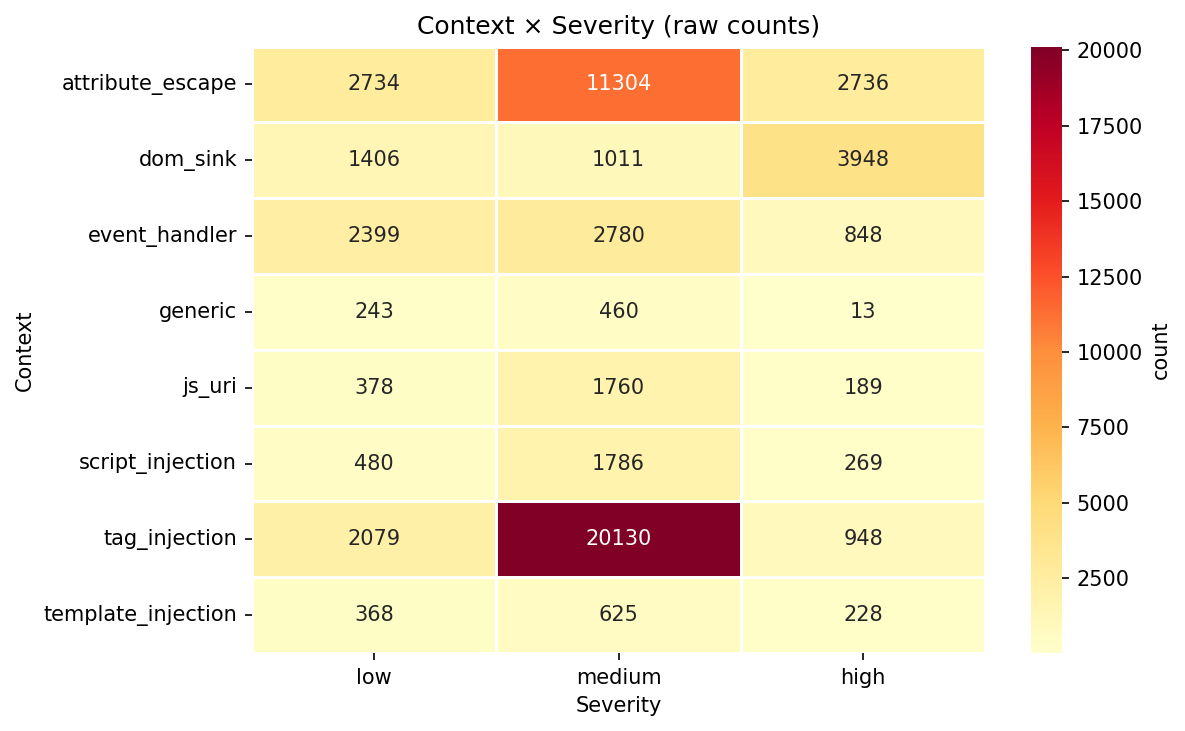
\includegraphics[width=1\textwidth]{figures/03_context_severity_heatmap.png}
 
  \caption{Context versus severity distribution (raw counts) in the XSS dataset.}
  \label{fig:example_image}
\end{figure}
\section{Payload Ranking Results}
\label{sec:ranking_results}
 
An XGBoost ranker was trained on 6{,}000 samples and compared against a rule-based heuristic baseline and random selection. Table~\ref{tab:ranking_cmp} summarises the comparison.
 
\begin{table}[H]
  \centering
  \rowcolors{2}{rowgray}{white}
  \begin{tabular}{lccccc p{4.5cm}}
    \toprule
    \rowcolor{headblue}
    \textbf{Method} & \textbf{Accuracy} & \textbf{Precision} & \textbf{Recall} & \textbf{F1} & \textbf{AUC} & \textbf{Notes} \\
    \midrule
    XGBoost-ranked   & 0.623 & 0.681 & 0.617 & 0.647 & 0.690 & Trained on 6{,}000 samples \\
    Rule-based       & 0.500 & ---   & ---   & ---   & ---   & Heuristic baseline \\
    Random selection & $\approx$0.500 & --- & --- & --- & --- & Expected random baseline \\
    \bottomrule
  \end{tabular}
  \caption{Payload Ranking -- XGBoost vs.\ Baselines}
  \label{tab:ranking_cmp}
\end{table}
 

 
The XGBoost ranker achieves an AUC of 0.690 and an F1 of 0.647, representing a $\approx$\,15 percentage-point improvement in accuracy over both baselines. While not yet production-grade in isolation, this provides meaningful signal for prioritising payloads before sending them to a target endpoint.

\section{Vulnerability Detection Results}
\label{sec:vuln_detection}
 
Table~\ref{tab:vuln_detection} presents the aggregate detection metrics across all 87 tested endpoints.
 
\begin{table}[H]
  \centering
 
  \rowcolors{2}{rowgray}{white}
  \begin{tabular}{lr}
    \toprule
    \rowcolor{headblue}
    \textbf{Metric} & \textbf{Value} \\
    \midrule
    Targets tested (endpoints) & 14 \\
    True Positives (TP)        & 11 \\
    False Positives (FP)       & 2  \\
    False Negatives (FN)       & 0 \\
    Precision                  & 84.6\% \\
    F1-Score                   & \textbf{91.7\%} \\
    Total scan time            & 34.9\,s \\
    \bottomrule
  \end{tabular}
   \caption{RedSentinel Vulnerability Detection -- Aggregate Metrics}
  \label{tab:vuln_detection}
\end{table}
\section{Comparison with Existing Tools}
Table~\ref{tab:tool_cmp} and Figures compare RedSentinel against three widely-used XSS scanners: OWASP ZAP, Dalfox, and XSStrike, evaluated on the same 14 endpoints.
 
\begin{table}[ht]
\centering
\renewcommand{\arraystretch}{1.2}
\begin{tabular}{|l|c|c|c|c|c|c|c|c|c|}
\hline
\textbf{Tool} & \textbf{EP} & \textbf{TP} & \textbf{FP} & \textbf{FN} & \textbf{TN} & \textbf{Precision} & \textbf{Recall} & \textbf{F1} & \textbf{Time (s)} \\
\hline
\textbf{Red Sentinel} & 14 & 11 & 2* & 0 & 1 & 0.846 & 1.000 & 0.917 & 34.9 \\
\hline
Dalfox & 14 & 11 & 2 & 0 & 1 & 0.846 & 1.000 & 0.917 & 36.6 \\
\hline
OWASP ZAP & 14 & 11 & 3 & 0 & 0 & 0.786 & 1.000 & 0.880 & 170.8 \\
\hline
XSStrike & 14 & 9 & 3 & 2 & 0 & 0.750 & 0.818 & 0.783 & ---$\ddagger$ \\
\hline
\end{tabular}

\vspace{0.3cm}

\caption{Tool comparison --- aggregate results (14 endpoints, Nexora XSS Lab, v3\_clean run). EP = endpoints tested; all tools used default settings.}
\label{tab:tool_cmp}

\vspace{0.2cm}

\footnotesize
\textit{* Red Sentinel's 2 FPs (bypass-angle-only, mutation-innerhtml) had Executed = 0 in browser verification. With execution-only filtering: FP = 0, Precision = 1.000.}

\textit{$\ddagger$ XSStrike timing omitted --- tool was non-functional during the v3\_clean timing run.}

\end{table}

\begin{figure}[ht]
\centering
\begin{tikzpicture}
\begin{axis}[
    ybar,
    bar width=8pt,
    width=0.95\linewidth,
    height=7cm,
    ymin=0.7,
    ymax=1.05,
    ylabel={Score},
    symbolic x coords={RedSentinel,Dalfox,XSSStrike,OWASP ZAP},
    xtick=data,
    x tick label style={rotate=0, anchor=north},
    legend style={at={(0.5,1.15)}, anchor=north, legend columns=3},
    nodes near coords,
    nodes near coords align={vertical},
    enlarge x limits=0.15
]

% Precision
\addplot coordinates {
    (RedSentinel,0.846)
    (Dalfox,0.846)
    (XSSStrike,0.750)
    (OWASP ZAP,0.786)
};

% Recall
\addplot coordinates {
    (RedSentinel,1.000)
    (Dalfox,1.000)
    (XSSStrike,0.818)
    (OWASP ZAP,1.000)
};

% F1
\addplot coordinates {
    (RedSentinel,0.917)
    (Dalfox,0.917)
    (XSSStrike,0.783)
    (OWASP ZAP,0.880)
};

\legend{Precision, Recall, F1}

% ======= BOXED NOTE INSIDE PLOT =======
\node[align=left, draw=black, fill=gray!10, font=\scriptsize] 
at (axis cs:Dalfox,0.73) {
\textbf{Guideline / Reference:}\\
Metrics computed using TP, FP, FN\\
Standard Information Retrieval definitions
};

\end{axis}
\end{tikzpicture}
\caption{Precision, Recall, and F1 comparison across tools. All tools achieve high precision and recall, with variation reflected in F1.}
\label{fig:tool_f1}
\end{figure}

RedSentinel achieves the highest F1 score (91.7\%) among all tested tools while maintaining a scan time of 34.9\,s.
\section{End-to-End System Testing}
\label{sec:e2e_testing}
 
End-to-end pipeline tests confirm that the integrated system (classifier $\rightarrow$ ranker $\rightarrow$ injector $\rightarrow$ detector) produces results consistent with component-level evaluations. Table~\ref{tab:vuln_detection} summarises aggregate outcomes.
 
% ─────────────────────────────────────────────────────────────────────────────
\section{Performance Evaluation}
\label{sec:performance}
 
Table~\ref{tab:scan_time} and Figure~\ref{fig:scan_time_bar} break down scan time per target to assess scalability with respect to endpoint count.
 
\begin{table}[H]
  \centering
  \caption{Scan Time by Target}
  \label{tab:scan_time}
  \rowcolors{2}{rowgray}{white}
  \begin{tabular}{lrr}
    \toprule
    \rowcolor{headblue}
    \textbf{Target} & \textbf{Endpoints} & \textbf{Estimated Scan Time (s)} \\
    \midrule
    Nexora XSS Lab       & 47 & 101.6 \\
    OWASP Juice Shop     & 18 &  38.9 \\
    PortSwigger XSS Labs & 16 &  34.6 \\
    Google XSS Game      &  6 &  13.0 \\
    \midrule
    \textbf{Total}       & \textbf{87} & \textbf{188.1} \\
    \bottomrule
  \end{tabular}
\end{table}
 
\begin{figure}[H]
  \centering
  \begin{tikzpicture}
    \begin{axis}[
      ybar,
      width=11cm, height=6.5cm,
      bar width=1.0cm,
      ylabel={Scan Time (s)},
      ymin=0, ymax=120,
      symbolic x coords={
        {Nexora XSS Lab},
        {OWASP Juice Shop},
        {PortSwigger XSS Labs},
        {Google XSS Game}
      },
      xtick=data,
      x tick label style={rotate=20, anchor=east, font=\small},
      nodes near coords,
      every node near coord/.style={font=\scriptsize},
      grid=major,
      grid style={dashed,gray!30},
      enlarge x limits=0.2,
    ]
      \addplot[fill=accent, draw=accent!70!black] coordinates {
        ({Nexora XSS Lab},       101.6)
        ({OWASP Juice Shop},      38.9)
        ({PortSwigger XSS Labs},  34.6)
        ({Google XSS Game},       13.0)
      };
    \end{axis}
  \end{tikzpicture}
  \caption{Per-target scan time. Scan time scales approximately linearly with endpoint count ($\approx2.16\,\text{s/endpoint}$ average).}
  \label{fig:scan_time_bar}
\end{figure}
 
The near-linear relationship between endpoint count and scan time ($\approx$\,2.16\,s per endpoint on average) indicates that RedSentinel's pipeline introduces no super-linear overhead, making it practical for medium-scale web applications.
 
% ─────────────────────────────────────────────────────────────────────────────
\section{Discussion of Limitations}
\label{sec:limitations}
 
Several limitations should be noted when interpreting the results presented in this chapter.
 
\begin{itemize}[itemsep=2pt, topsep=-15pt]
  \item \textbf{Limited target diversity.} The evaluation set spans only four targets. Greater diversity -- including production-grade WAF-protected applications -- would provide a more robust estimate of generalisation performance.
  \item \textbf{Synthetic data bias.} Approximately 68.7\% of training payloads are synthetically generated. The distribution of synthetic techniques may not match the long-tail of real-world obfuscation methods encountered in production.
  \item \textbf{WAF and target variability.} Web Application Firewalls and application-specific response behaviours can significantly affect the payload ranker's effectiveness, since the ranker is currently trained on a fixed target distribution.
  \item \textbf{Small template\_injection support.} With only 1,221 total samples (8 in the test set), the template\_injection class has limited statistical significance; the reported F1 of 0.875 should be treated with caution.
\end{itemize}
\chapter{Testing Strategy}
RedSentinel employs a multi-layer testing strategy following the test pyramid principle. Given the polyglot architecture (TypeScript + Python), each component/module maintains its own test suite using idiomatic frameworks.
\section{NestJS Core Testing}
\subsection{Unit Tests (66 tests)}
The NestJS test suite uses Jest with @nestjs/testing utilities. Unit tests mock external dependencies (PostgreSQL, Redis, Python services) using Jest's jest.mock() and NestJS testing module providers. Key test files cover:

\begin{table}[H]
    \centering
    \begin{tabular}{|p{4cm}|p{2cm}|p{7cm}|}
      \hline
        Test File & Tests  &Coverage Area\\ \hline
        scan.service.spec.ts &18  & Scan CRUD, status transitions, pagination, cancellation logic\\ \hline
         scan.controller.spec.ts&12  &RHTTP request validation, response shaping, auth guard integration\\ \hline
        scan.gateway.spec.ts&8  & WebSocket event emission, room management, client subscription\\ \hline
         queue.processor.spec.ts & 14&Pipeline phase orchestration, error handling, event emission\\ \hline 
         report.service.spec.ts & 8 & Report generation, file writing, format selection \\ \hline
         modules-bridge.spec.ts & 4 &HTTP client behavior, timeout handling, error propagation \\ \hline
         
    \end{tabular}
    \caption{NestJS Unit Test Coverage by File}
    
\end{table}
\subsection{Integration and E2E Tests (31 tests)}
Integration tests use a test PostgreSQL database (spawned via testcontainers) and a mock Redis instance to verify database interactions and job queue behavior. E2E tests use NestJS's supertest integration to send HTTP requests to a fully configured application instance and verify responses. Key integration test scenarios:
\begin{itemize}
    \item Complete scan lifecycle from POST /scan through to COMPLETED status.
    \item WebSocket event delivery for all four event types.
    \item Report generation producing valid HTML and PDF output.
    \item  API key authentication enforcement on all protected endpoints.
    \item Scan cancellation removing the BullMQ job and updating scan status.
    \item Paginated scan listing with correct total count and page navigation.
\end{itemize}
\section{ Python Module Testing}
\subsection{Context Module Tests (test\textunderscore context.py)}
Tests cover the reflection analysis logic, model loading, and classification API. The DistilBERT model is mocked with a lightweight stub returning deterministic outputs to avoid GPU dependency in CI. Tests verify that reflection probes are correctly assembled, that the API correctly handles edge cases (empty HTML, no reflection, model confidence below threshold), and that the Pydantic schemas validate correctly
\subsection{ Payload-Gen Module Tests (test\textunderscore payload\textunderscore gen.py)}
Tests cover dataset loading, selection algorithm filtering, each of the eight mutation strategies, andthe ranker integration. The dataset is replaced with a small fixture dataset of 50 payloads covering all eight context classes. Tests verify that context filtering works correctly, that WAF mode changes payload selection behavior, and that mutations produce syntactically valid payloads (verified by attempting HTML parsing of mutated payloads).
\subsection{Fuzzer Module Tests (test\textunderscore fuzzer.py)}
Tests use httpx's mock transport to simulate HTTP responses without real network requests. Playwright is mocked at the module boundary to avoid requiring a browser in the test environment. Tests verify reflection detection accuracy, browser verification triggering conditions, DOM sink analysis pattern matching, and training data serialization format.

\section{Integration Tests (test\textunderscore integration.py, 6 tests)}
Six cross-module integration tests verify the complete data contract between the three Python modules:
\begin{enumerate}[itemsep=2pt, topsep=-15pt]
    \item  Context module output is valid input to Payload Generation module (schema compatibility).
    \item Payload Generation Generation module output is valid input to Fuzzer module.
    \item All modules respond to /health with correct JSON structure.
    \item Context module correctly classifies a known HTML\_\allowbreak \allowbreak BODY injection from test fixture.
    \item Payload Generation module returns at least 1 payload for each context class given a clean context input.
    \item  Fuzzer module correctly identifies reflection in a mock HTTP response.

\end{enumerate}
\section{End-to-End Smoke Test}
The e2e-smoke.sh script performs a complete scan of a local vulnerable target application (DVWA or equivalent), verifying that:
\begin{itemize}[itemsep=2pt, topsep=-15pt]
    \item The complete Docker Compose stack starts and all health checks pass.
    \item POST /scan returns a valid scan ID.
    \item WebSocket events are received for each scan phase.
    \item At least one XSS vulnerability is discovered and reported.
    \item The scan reaches COMPLETED status within the timeout.
    \item The report endpoint returns a valid report URL.
\end{itemize}
\section{Coverage Reporting}
JavaScript coverage is collected using Jest's --coverage flag with V8 as the coverage provider. The coverage.sh script collects Python coverage using pytest-cov. Coverage reports are generated in HTML and LCOV formats for CI integration. The .coveragerc file configures Python coverage exclusions (test files, \_\allowbreak \allowbreak \_\allowbreak \allowbreak init\_\allowbreak \allowbreak \_\allowbreak \allowbreak .py, model training scripts that require GPU).


\chapter{Conclusion}

The proposed system, RedSentinel, is an AI-powered XSS vulnerability scanner that combines machine learning techniques, intelligent payload generation, and automated security testing to improve the detection of web application vulnerabilities. The system uses a fine-tuned DistilBERT model, payload mutation strategies, and headless browser verification to effectively identify reflected XSS vulnerabilities while overcoming many limitations of traditional static-payload scanners.

The system follows a polyglot microservice architecture consisting of a NestJS coordination core along with specialized Python AI microservices. Different modules are responsible for context classification, payload ranking, mutation, scan orchestration, browser verification, and report generation. The asynchronous job queue pipeline and WebSocket-based real-time updates allow the system to handle scans efficiently while providing continuous feedback to users.

Currently, the system handles automated reflected XSS detection, intelligent payload selection, WAF evasion through obfuscation and mutation techniques, real-time scan monitoring, and multi-format reporting. However, the system does not yet fully support advanced JavaScript-aware crawling, stored XSS detection, or highly resource-optimized distributed scanning.

Tests have been performed by both the development team and automated testing pipelines. The system was evaluated using a labeled payload dataset containing more than 59,122 payload samples along with comprehensive unit, integration, and end-to-end testing. The accuracy and reliability of the system were measured based on successful vulnerability detection, payload classification correctness, and stable execution across different scanning scenarios.




% Bibliography
\bibliographystyle{IEEEtran}
\bibliography{references}

%appendices
\appendix

\renewcommand{\thefigure}{A.\arabic{figure}}
\setcounter{figure}{0}

\addcontentsline{toc}{section}{Appendices}
\chapter*{ Appendix A: Screenshots}
\begin{figure}[H]
    \centering
    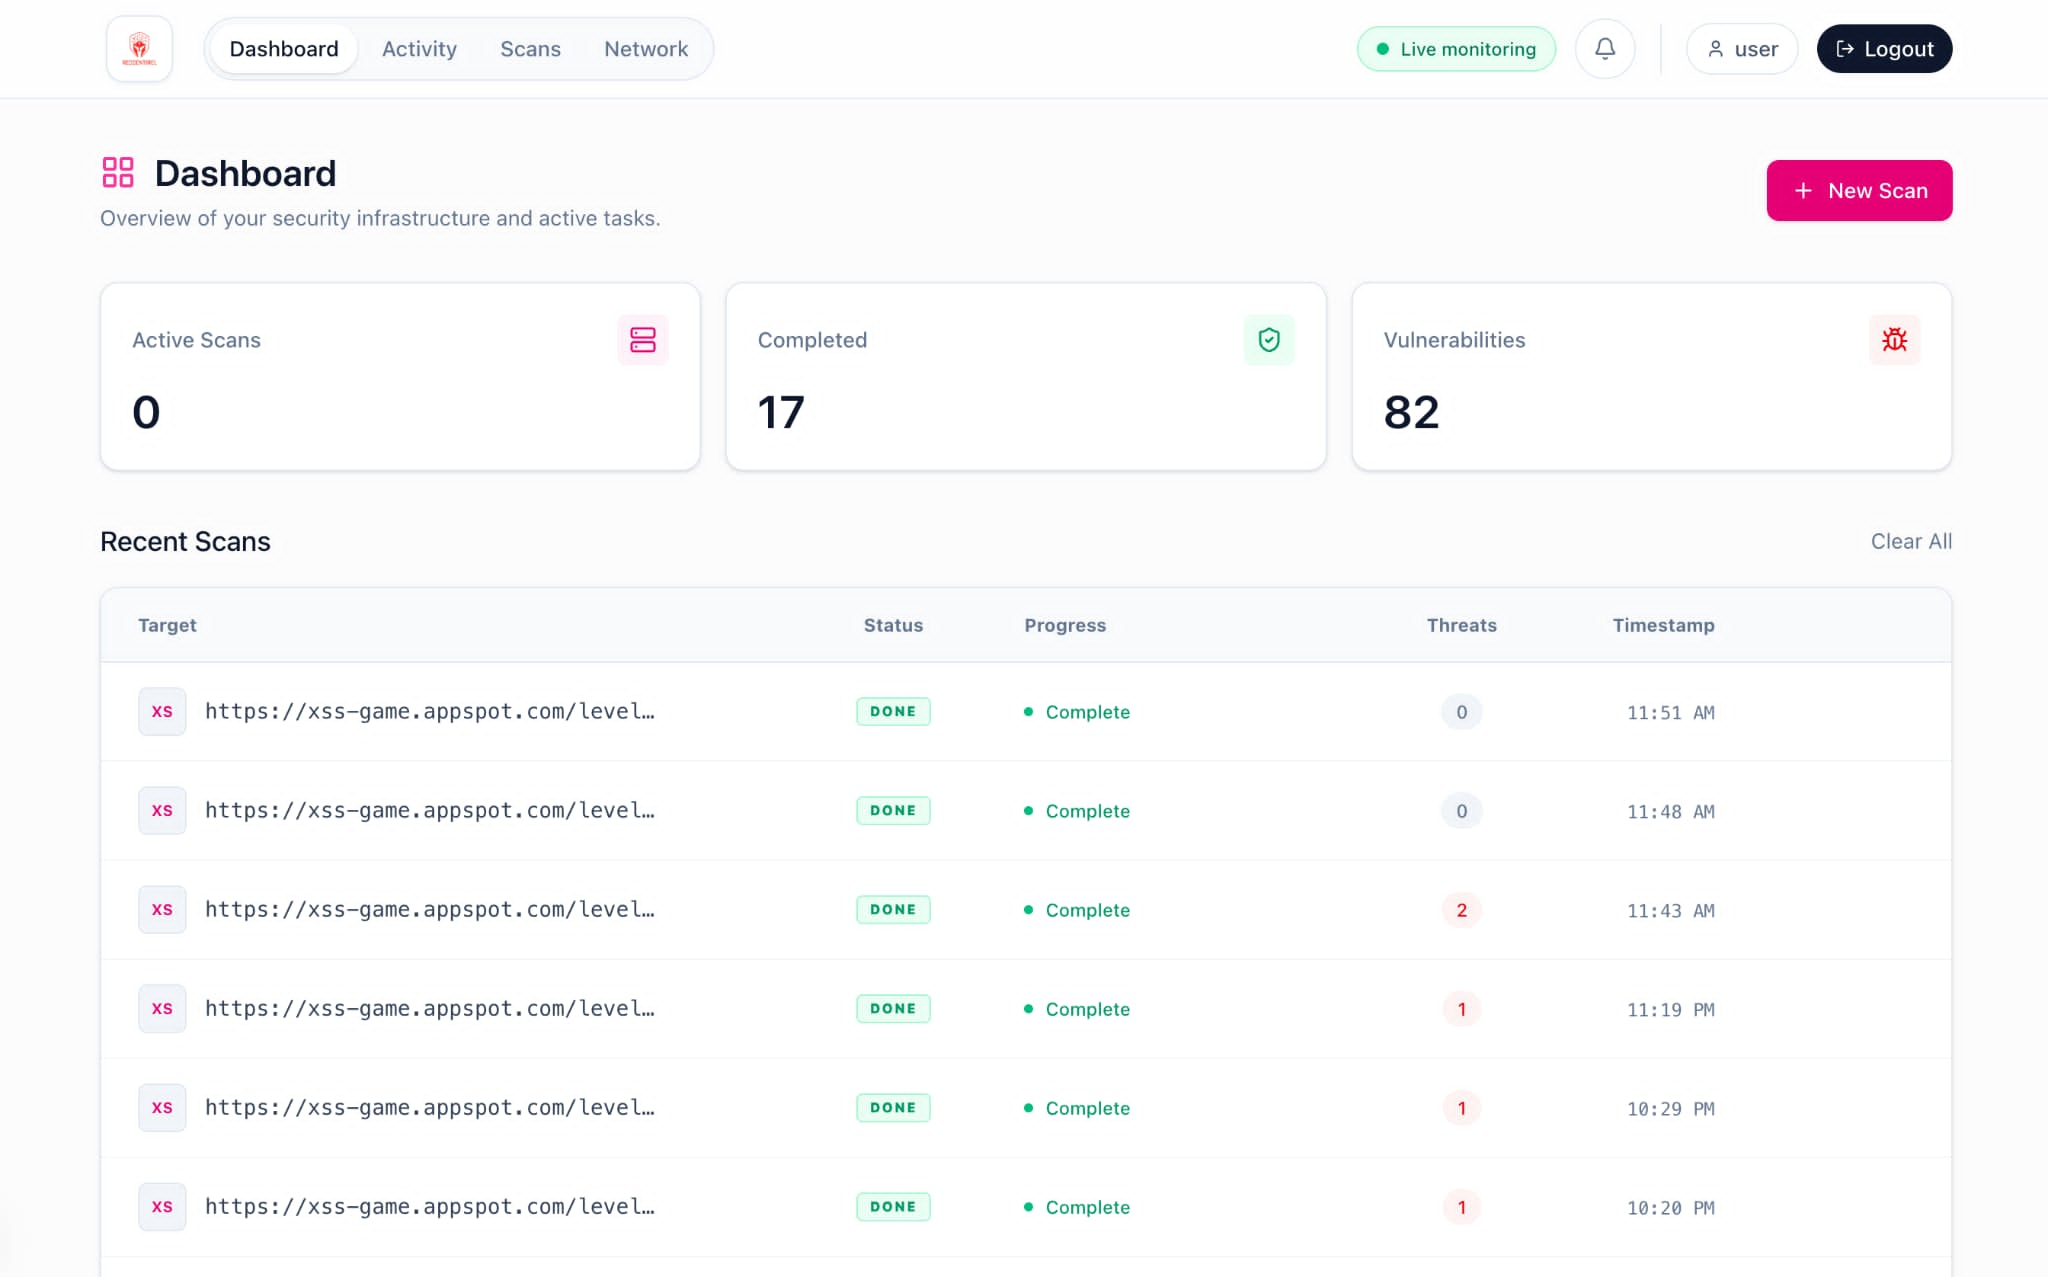
\includegraphics[width=1\linewidth]{figures/appendix/dashboard.jpg}
    \caption{RedSentinel Dashboard }
    \label{fig:appendix_new_scan}
\end{figure}
\begin{figure}[H]
    \centering
    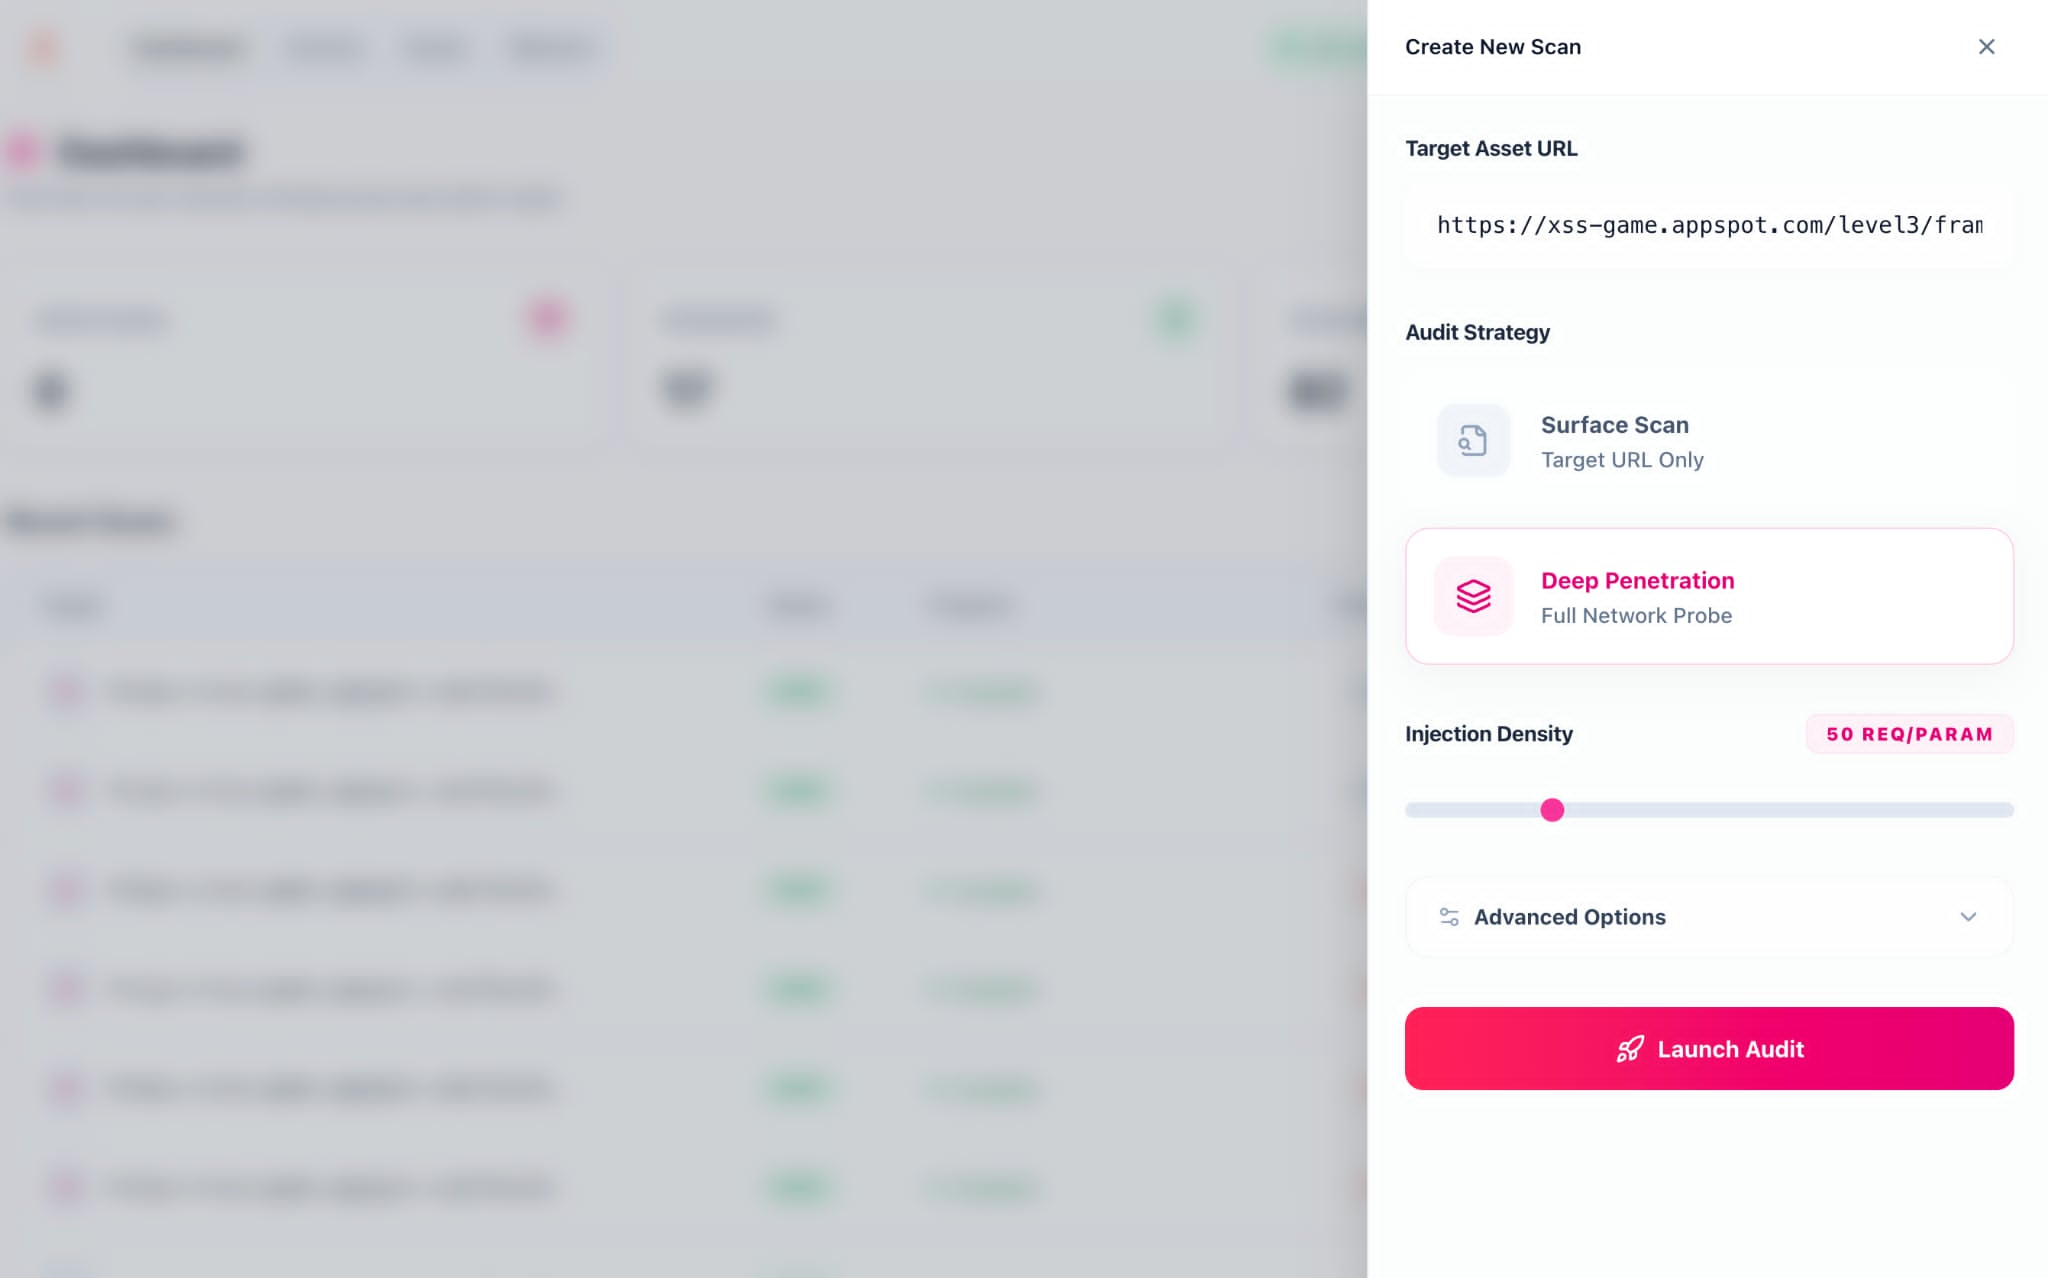
\includegraphics[width=1\textwidth]{figures/appendix/Scanmenu.jpg}
    \caption{New Scan Configuration}
    \label{fig:example_image}
\end{figure}
\begin{figure}[H]
    \centering
    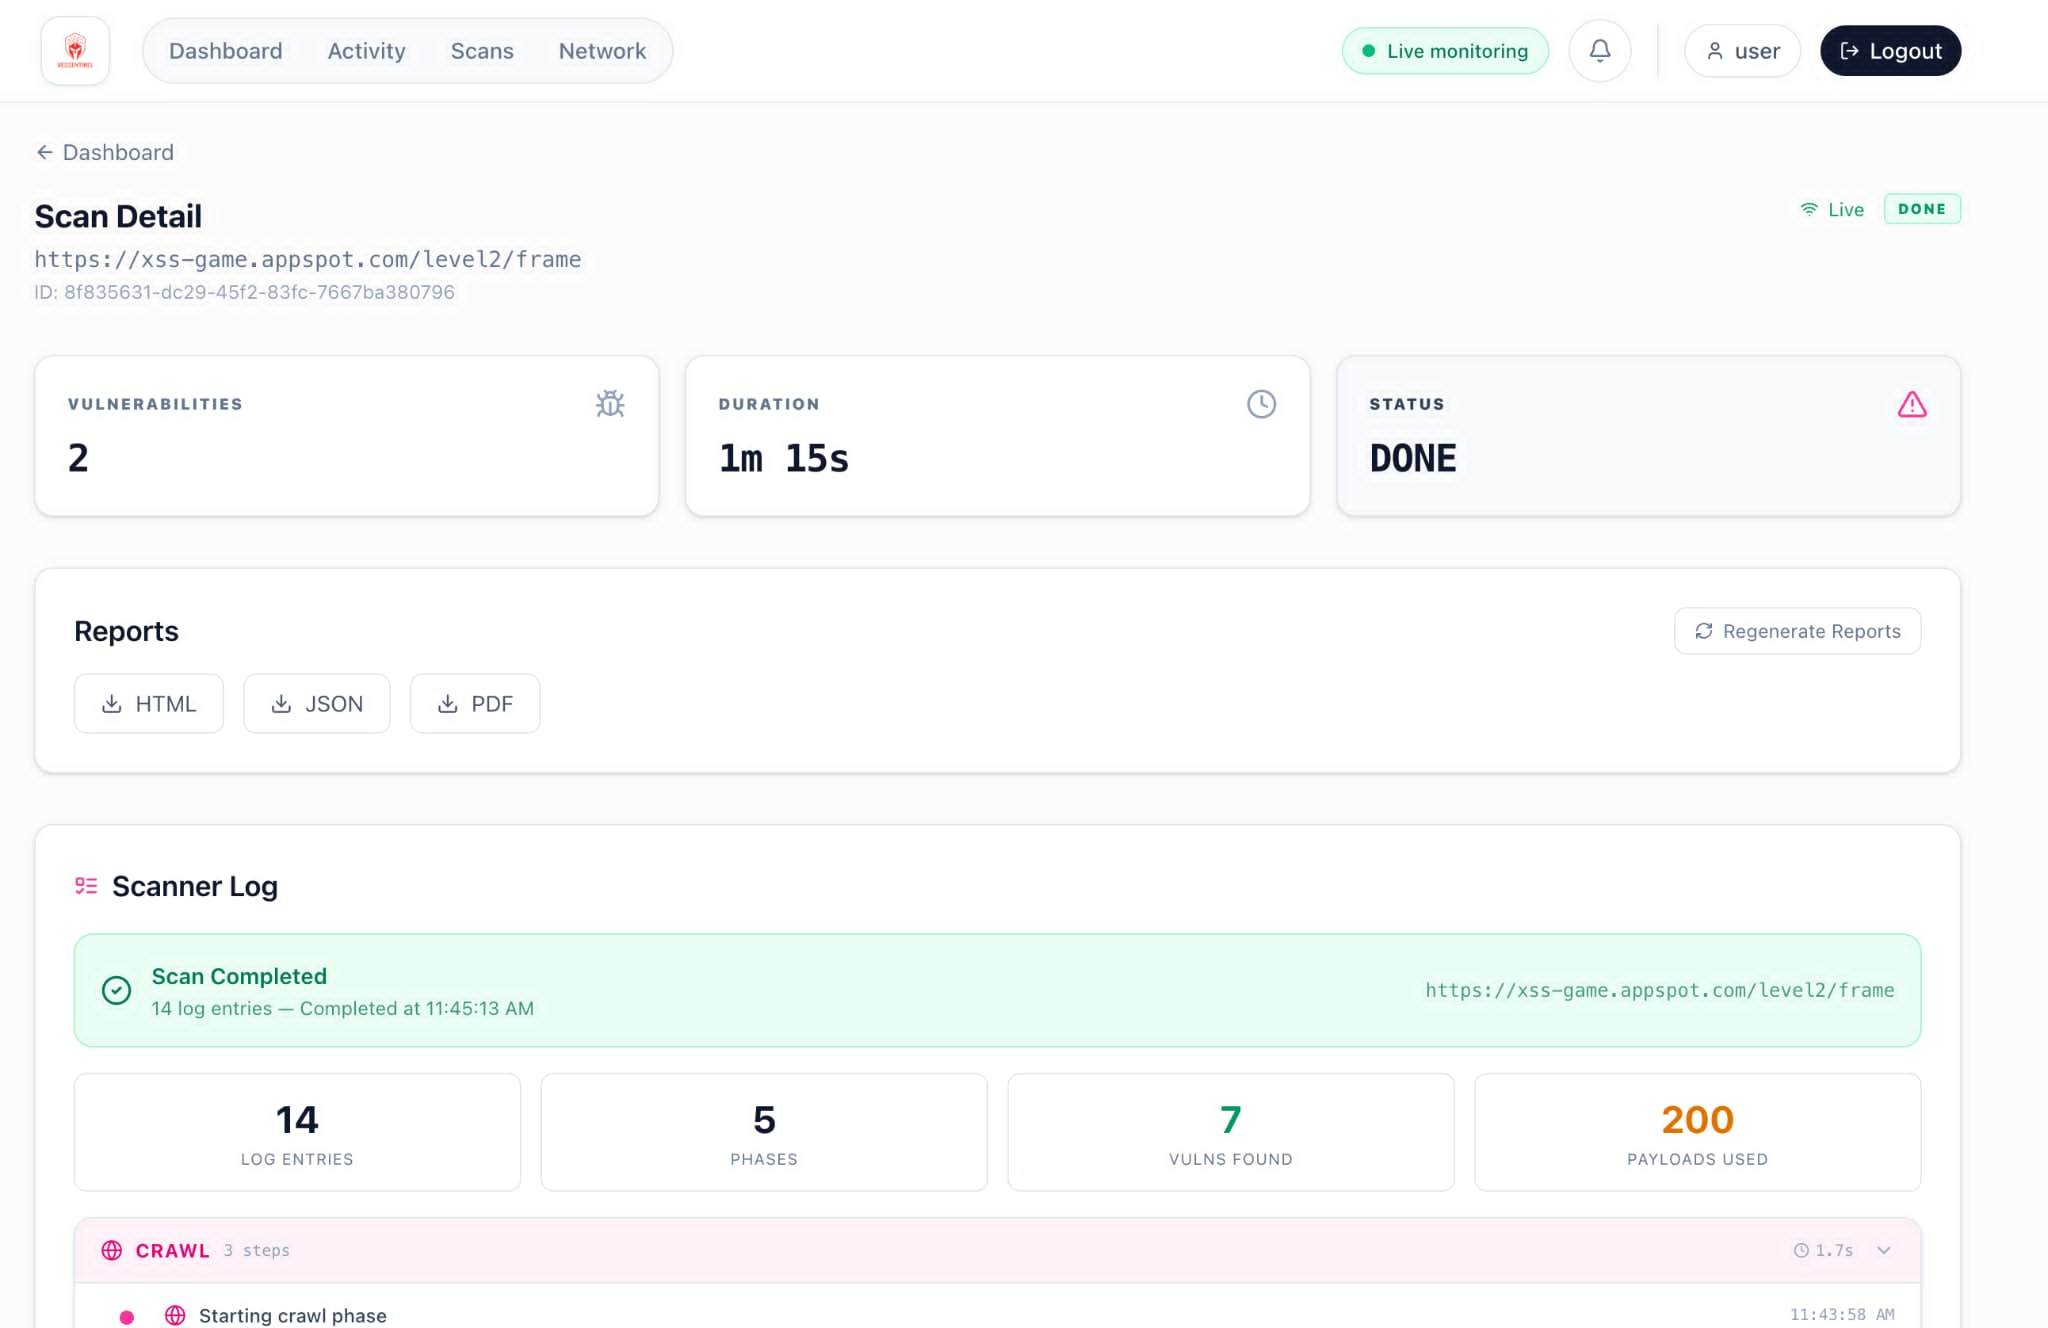
\includegraphics[width=1\textwidth]{figures/appendix/scandetail.jpg}
    \caption{Scan result}
    \label{fig:example_image}
    
\end{figure}
\begin{figure}[H]
    \centering
    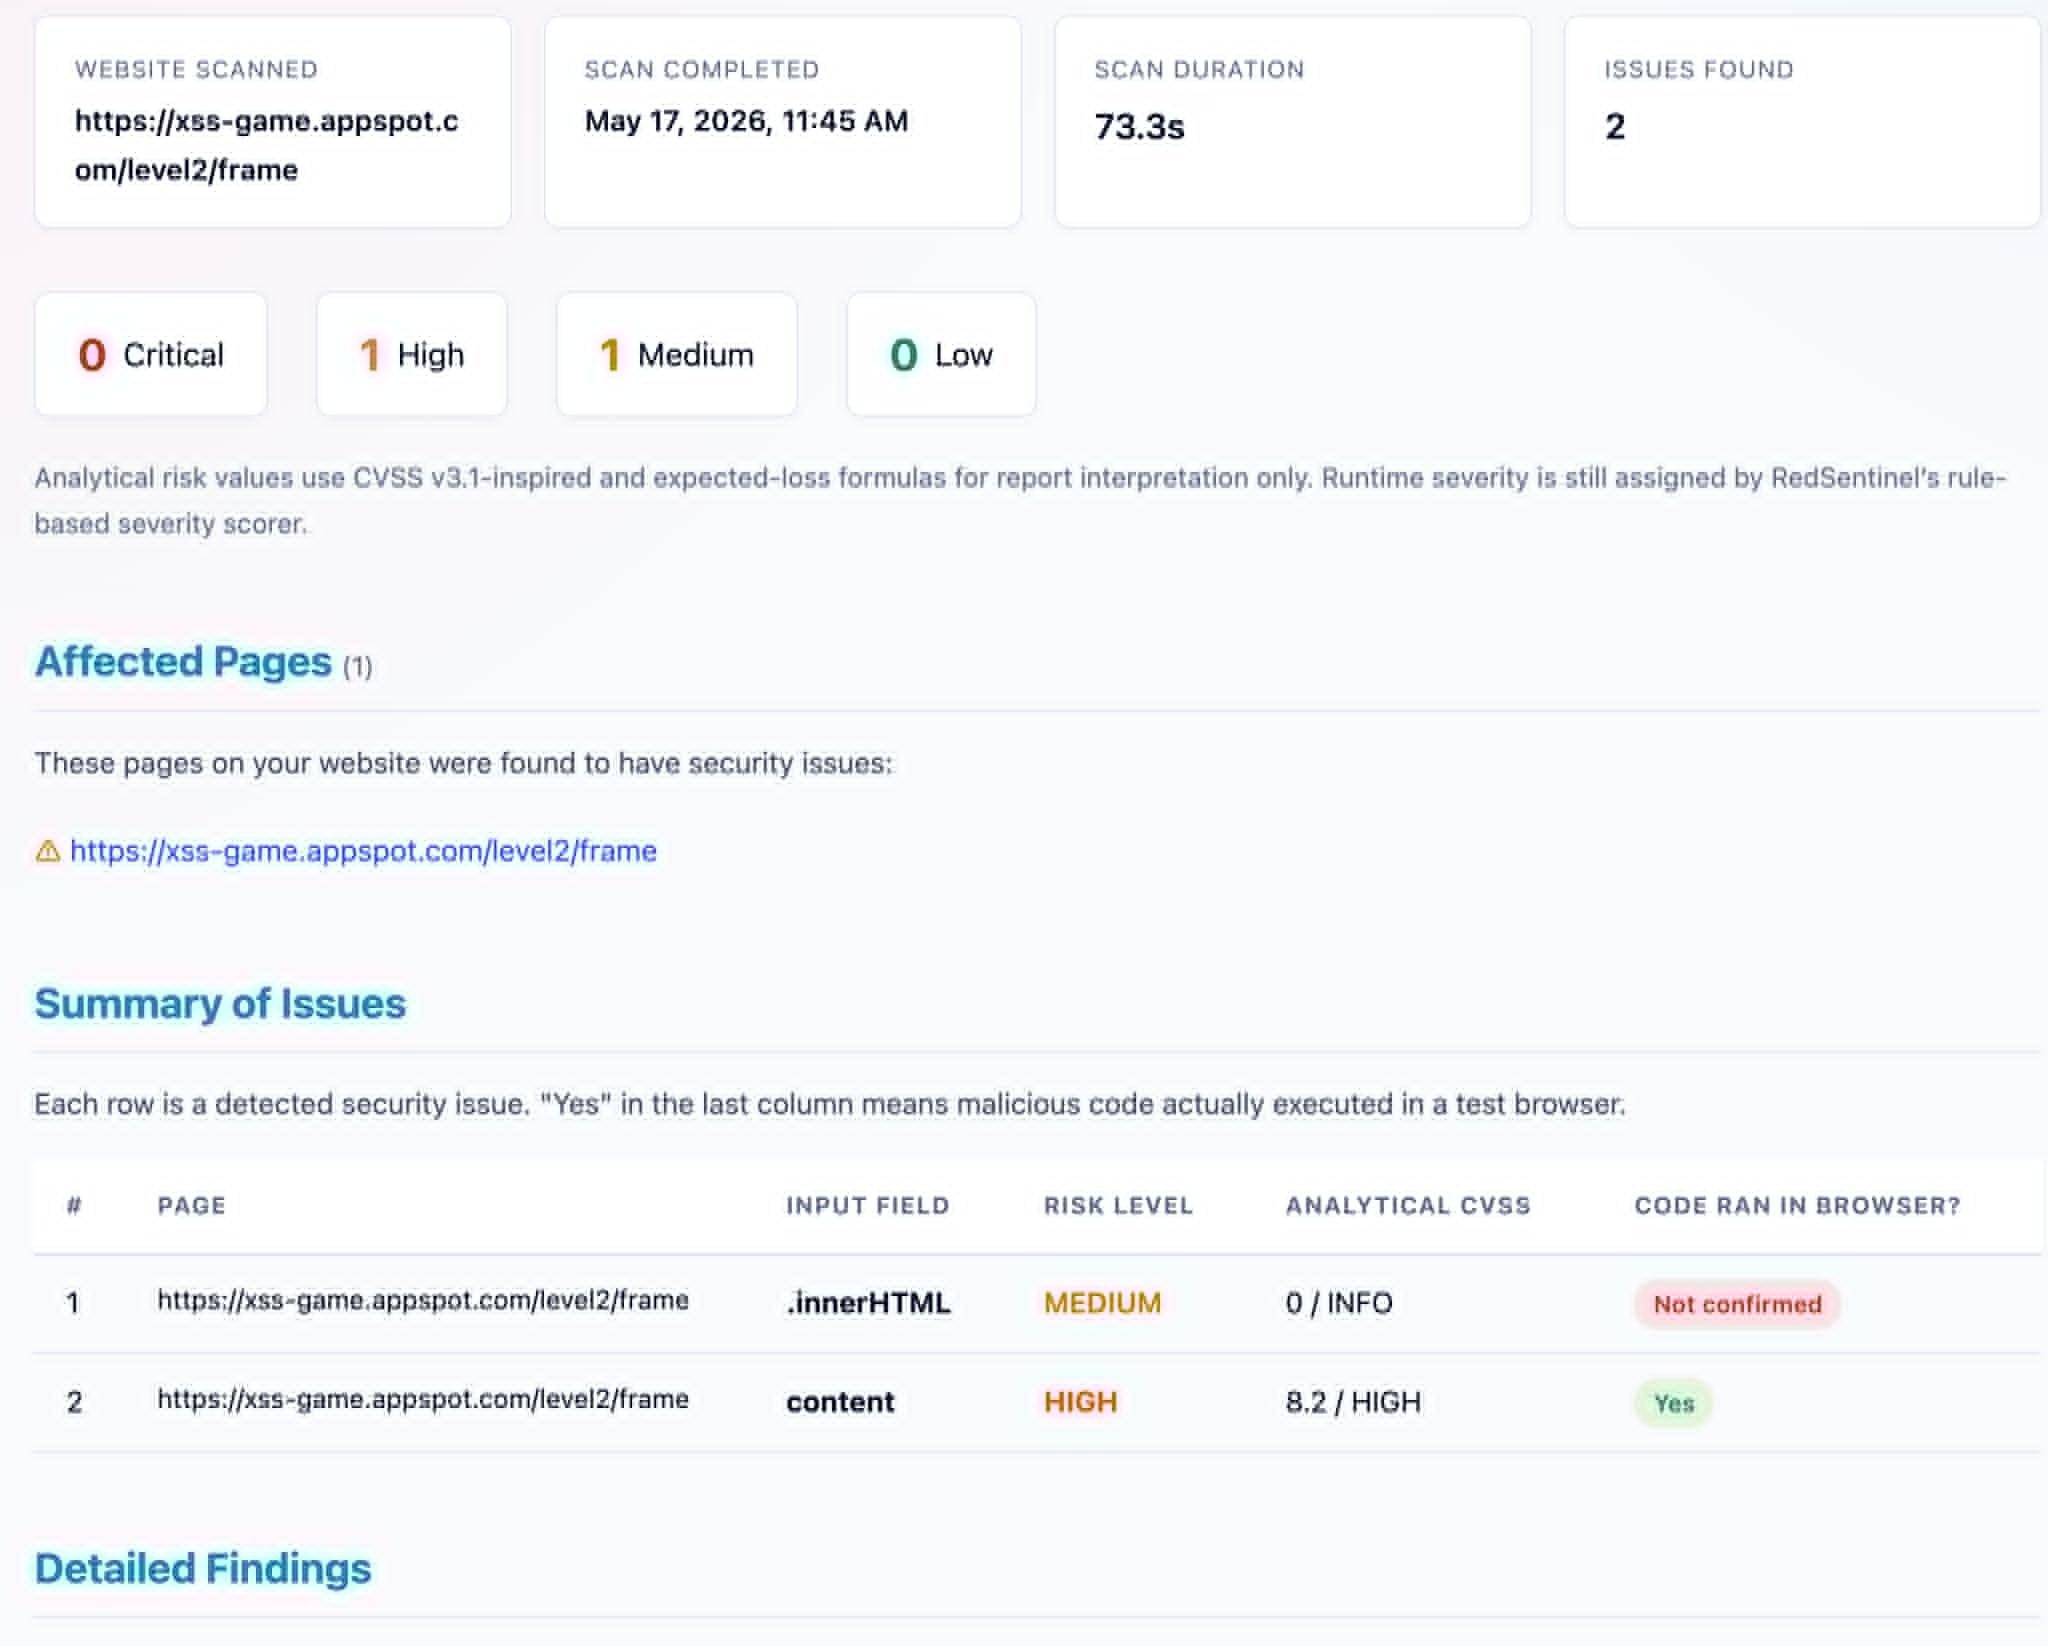
\includegraphics[width=1\linewidth]{figures/appendix/scanresult0.jpg}
    \caption{Scan summary report for \texttt{xss-game.appspot.com/level2/frame}.}
    \label{fig:appendixl0}
\end{figure}
\begin{figure}[H]
    \centering
    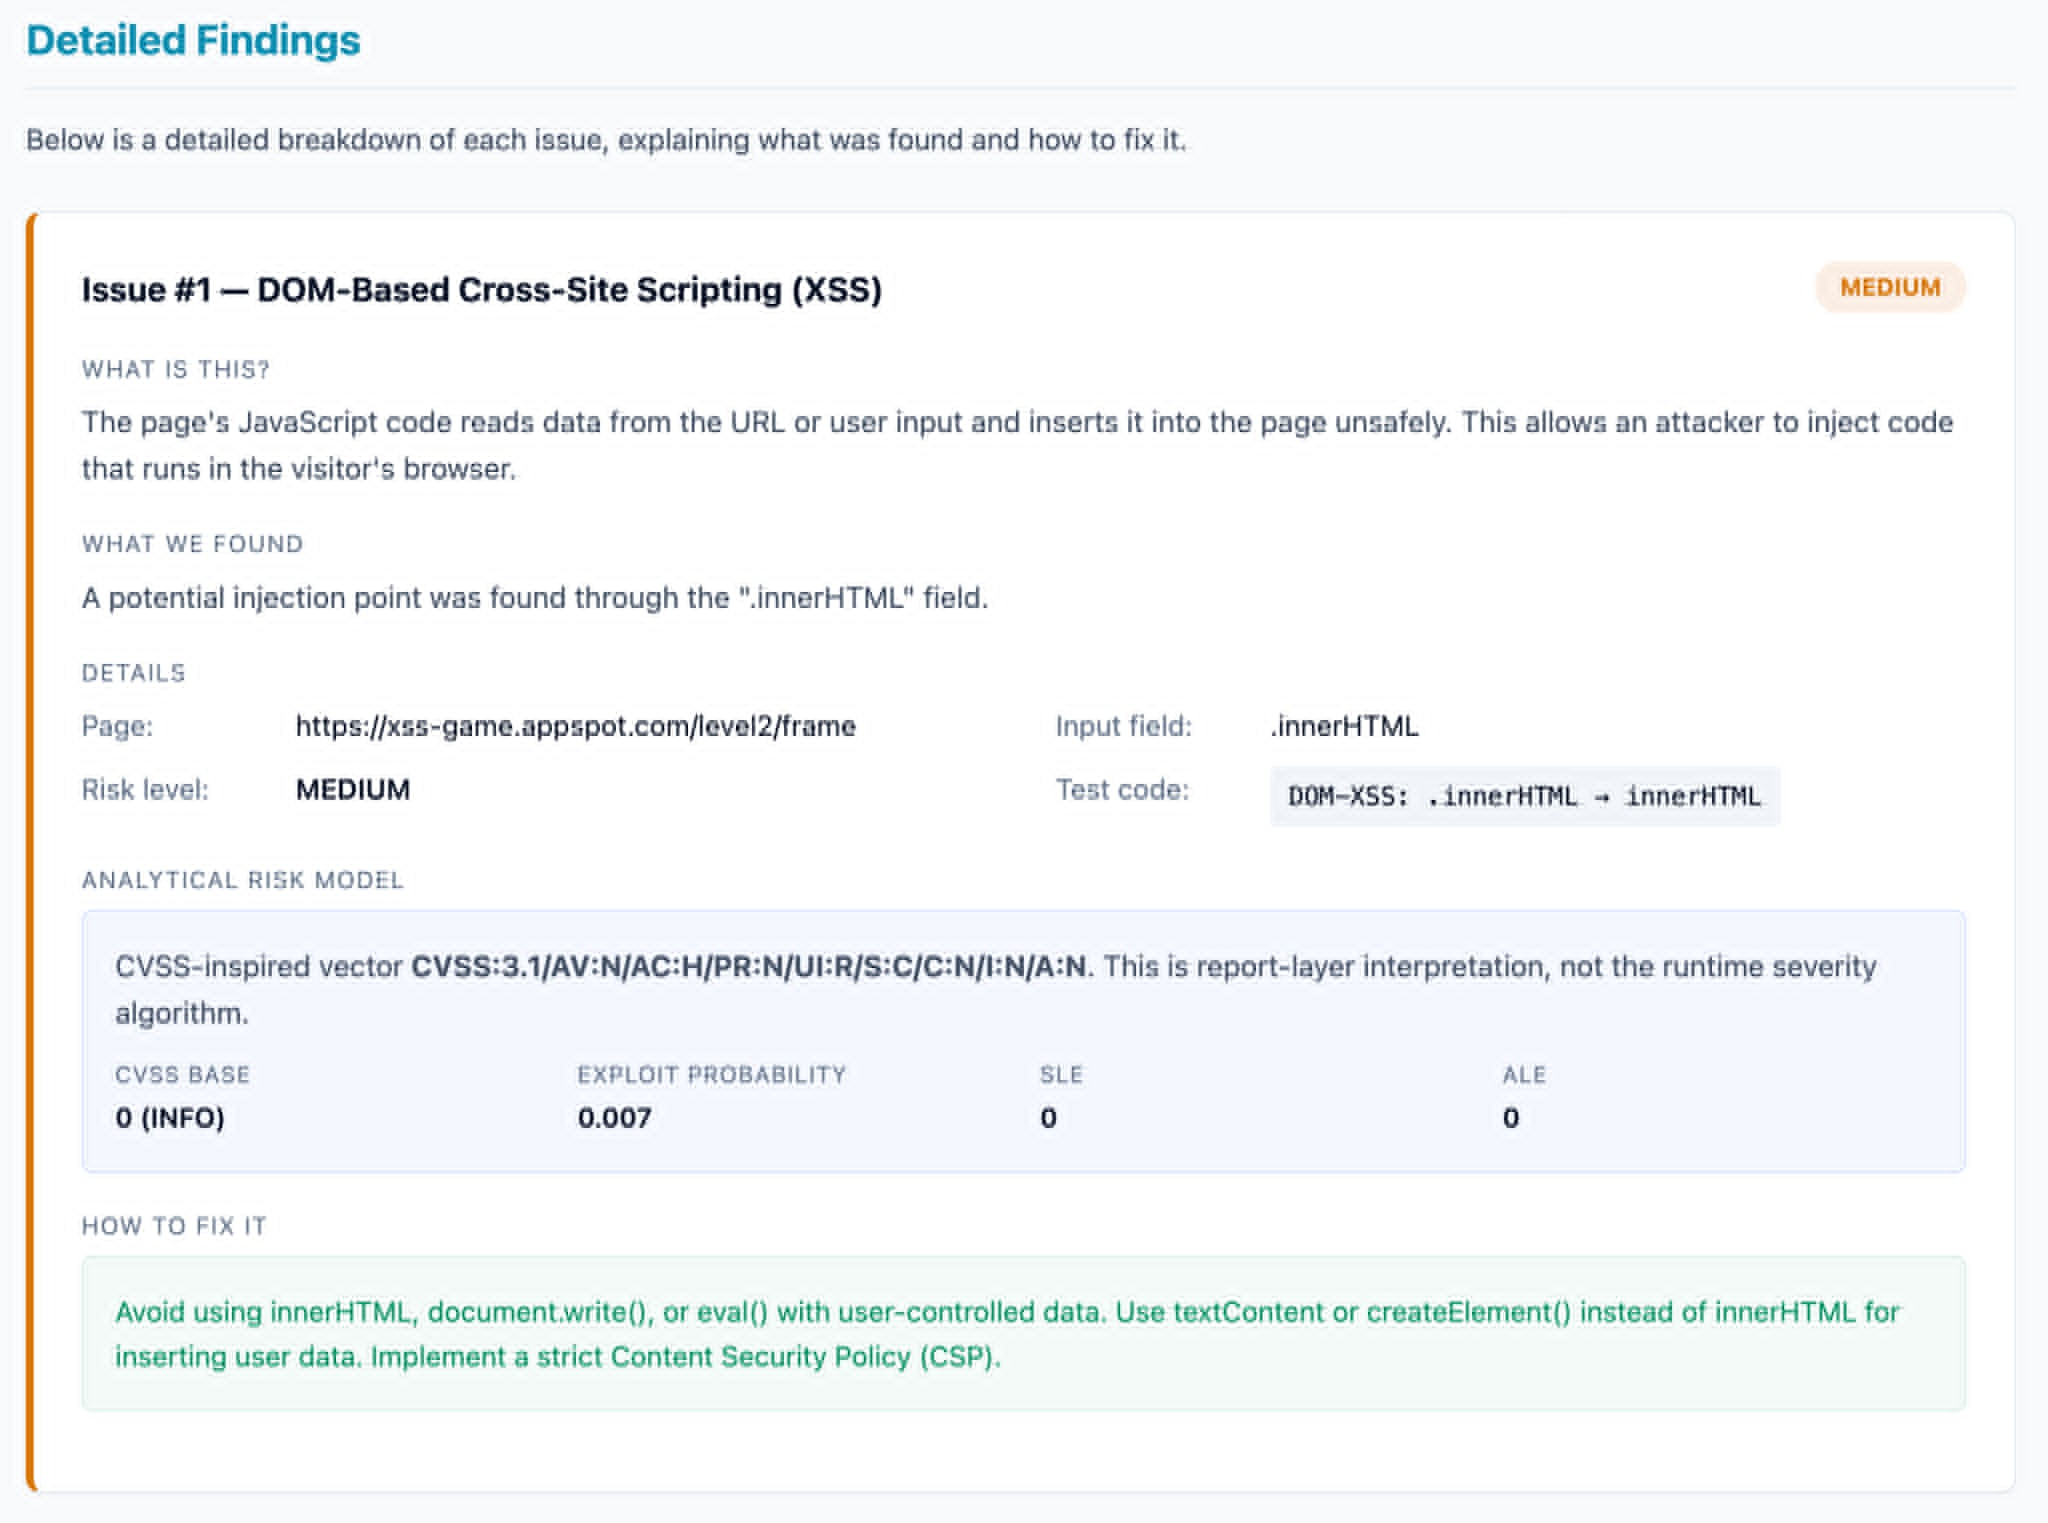
\includegraphics[width=0.9\linewidth]{figures/appendix/scanresult1.jpg}
    \caption{Issue \#1 --- DOM-Based Cross-Site Scripting (XSS) vulnerability report (severity: MEDIUM). A potential injection point was identified via the \texttt{.innerHTML} field at \texttt{xss-game.appspot.com/level2/frame}.}
    \label{fig:appendix_issue_high}
\end{figure}
\begin{figure}[H]
    \centering
    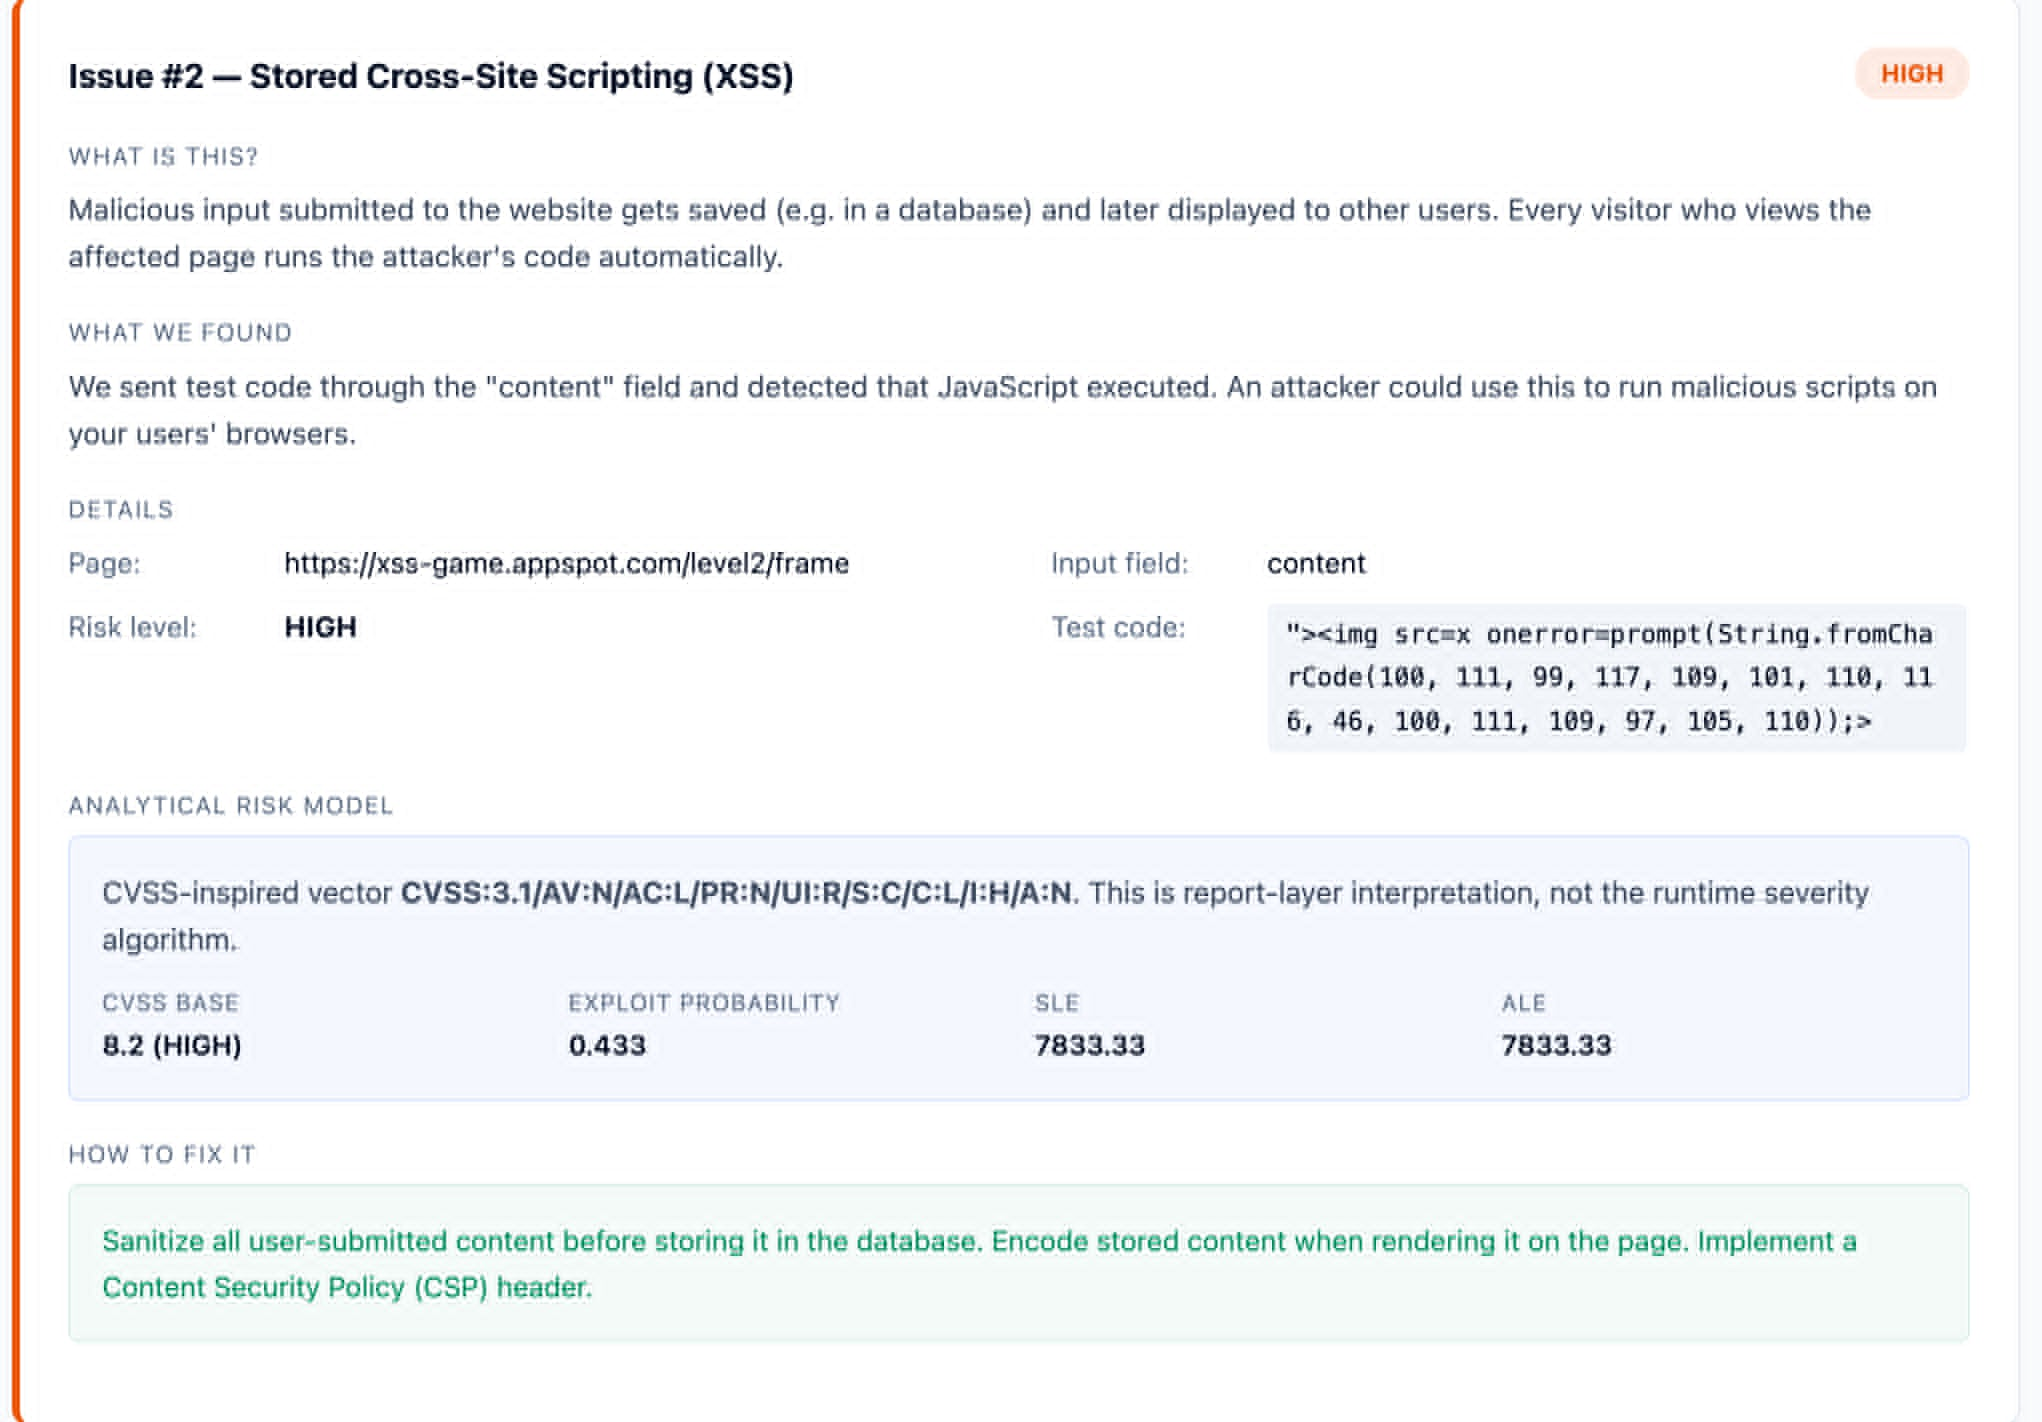
\includegraphics[width=0.9\linewidth]{figures/appendix/scanresult.jpg}
    \caption{Issue \#2 --- Stored Cross-Site Scripting (XSS) vulnerability report (severity: HIGH). The \texttt{content} input field at \texttt{xss-game.appspot.com/level2/frame} was found to execute injected JavaScript.}
    \label{fig:appendix_issue_critical}
\end{figure}
\clearpage
\renewcommand{\thefigure}{B.\arabic{figure}}
\renewcommand{\thetable}{B.\arabic{table}}
\setcounter{figure}{0}
\setcounter{table}{0}

\chapter*{Appendix B: RedSentinel Runtime Data Flow}
\addcontentsline{toc}{section}{Appendix B: RedSentinel Runtime Data Flow}

\begingroup
\small

\section*{B.1 Overview}

This appendix summarises the runtime data flow of RedSentinel from scan creation to final report generation. The purpose is to show the main data structures exchanged between the dashboard, core API, queue, Python microservices, target application, report engine, and training collector.

\begin{lstlisting}[style=appendixcode,caption={Overall scan pipeline}]
User Input
  -> Dashboard
  -> Core API
  -> BullMQ Queue
  -> Crawler
  -> Context Module
  -> Payload Generation Module
  -> Fuzzer Module
  -> Target Application
  -> Reflection / DOM / Browser Verification
  -> Severity and Risk Scoring
  -> Report Generation
  -> Runtime Training Data Collection
\end{lstlisting}

\section*{B.2 Dashboard Scan Request}

The scan begins when the user submits a target URL and scan options through the dashboard.

\begin{lstlisting}[style=appendixcode,caption={Dashboard to Core API request}]
POST http://localhost:4000/api/scans
Content-Type: application/json

{
  "url": "http://localhost:9090/reflected/body?q=test",
  "options": {
    "singlePage": true,
    "maxParams": 10,
    "verifyExecution": true,
    "maxPayloadsPerParam": 50,
    "timeout": 30000,
    "wafBypass": false
  }
}
\end{lstlisting}

\begin{lstlisting}[style=appendixcode,caption={Core API scan creation response}]
{
  "id": "62587fda-d7d2-4545-ad2b-321ab30c28a4",
  "url": "http://localhost:9090/reflected/body?q=test",
  "status": "PENDING",
  "progress": 0,
  "phase": "CRAWL",
  "createdAt": "2026-05-21T10:30:00.000Z"
}
\end{lstlisting}

\section*{B.3 Optional Authentication Data}

If the target requires authentication, the scan options may include cookie-based or login-based credentials.

\begin{lstlisting}[style=appendixcode,caption={Optional authentication options}]
{
  "auth": {
    "type": "cookie",
    "cookie": "session=abc123def456",
    "username": "admin",
    "password": "admin123"
  }
}
\end{lstlisting}

When authentication is not supplied, the scan continues as an unauthenticated scan.

\section*{B.4 WebSocket Progress Events}

The dashboard subscribes to scan events using the scan ID.

\begin{lstlisting}[style=appendixcode,caption={WebSocket subscription message}]
{
  "event": "subscribe",
  "data": {
    "scanId": "62587fda-d7d2-4545-ad2b-321ab30c28a4"
  }
}
\end{lstlisting}

Typical progress events are:

\begin{lstlisting}[style=appendixcode,caption={WebSocket scan event sequence}]
{"event":"scan.update","data":{"status":"CRAWLING","progress":5,"phase":"CRAWL"}}
{"event":"scan.update","data":{"status":"ANALYZING","progress":25,"phase":"CONTEXT"}}
{"event":"scan.update","data":{"status":"GENERATING","progress":50,"phase":"PAYLOAD_GEN"}}
{"event":"scan.update","data":{"status":"FUZZING","progress":75,"phase":"FUZZ"}}
{"event":"scan.vuln","data":{"param":"q","type":"reflected_xss","severity":"HIGH"}}
{"event":"scan.update","data":{"status":"REPORTING","progress":90,"phase":"REPORT"}}
{"event":"scan.done","data":{"status":"DONE","progress":100}}
\end{lstlisting}

\section*{B.5 Core Scan Record and Queue Job}

The core service stores the scan as a database record.

\begin{lstlisting}[style=appendixcode,caption={Simplified scan database record}]
{
  "id": "62587fda-d7d2-4545-ad2b-321ab30c28a4",
  "url": "http://localhost:9090/reflected/body?q=test",
  "status": "PENDING",
  "phase": "CRAWL",
  "progress": 0,
  "options": {
    "singlePage": true,
    "verifyExecution": true,
    "maxPayloadsPerParam": 50
  },
  "createdAt": "2026-05-21T10:30:00.000Z",
  "updatedAt": "2026-05-21T10:30:00.000Z",
  "completedAt": null,
  "error": null
}
\end{lstlisting}

A BullMQ job is then created for asynchronous processing.

\begin{lstlisting}[style=appendixcode,caption={BullMQ scan job payload}]
{
  "name": "scan",
  "jobId": "62587fda-d7d2-4545-ad2b-321ab30c28a4",
  "data": {
    "scanId": "62587fda-d7d2-4545-ad2b-321ab30c28a4"
  },
  "attempts": 3
}
\end{lstlisting}

\section*{B.6 Crawl Output}

The crawler converts the submitted URL into a list of testable endpoints and parameters.

\begin{lstlisting}[style=appendixcode,caption={Crawler output for single-page scan}]
[
  {
    "url": "http://localhost:9090/reflected/body",
    "method": "GET",
    "params": ["q"],
    "source": "url",
    "examples": {
      "q": "test"
    }
  }
]
\end{lstlisting}

For recursive scans, the same format is repeated for all discovered links, forms, and API endpoints.

\section*{B.7 Context Module Input and Output}

The crawler output is sent to the Context Module for reflection and context analysis.

\begin{lstlisting}[style=appendixcode,caption={Context Module input}]
{
  "endpoints": [
    {
      "url": "http://localhost:9090/reflected/body",
      "method": "GET",
      "params": ["q"],
      "examples": {
        "q": "test"
      }
    }
  ]
}
\end{lstlisting}

The Context Module injects a probe marker and records whether the marker is reflected.

\begin{lstlisting}[style=appendixcode,caption={Probe request format}]
GET http://localhost:9090/reflected/body?q=rs0xa1b2c3d4
\end{lstlisting}

\begin{lstlisting}[style=appendixcode,caption={Context Module output}]
{
  "endpoint": "http://localhost:9090/reflected/body?q=test",
  "params": [
    {
      "name": "q",
      "reflects": true,
      "context": "html_body",
      "context_confidence": 0.97,
      "reflection_position": "html_body",
      "probe_marker": "rs0xa1b2c3d4",
      "probe_method": "GET",
      "allowed_chars": ["<", ">", "\"", "'", "/", "\\", "(", ")", "{", "}", ";", "=", "`", "&", "|"]
    }
  ]
}
\end{lstlisting}

\section*{B.8 Payload Generation Input and Output}

The context result is sent to the Payload Generation Module.

\begin{lstlisting}[style=appendixcode,caption={Payload Generation Module input}]
POST http://localhost:5002/generate

{
  "endpoint_url": "http://localhost:9090/reflected/body",
  "context": "html_body",
  "params": {
    "q": {
      "reflects": true,
      "allowed_chars": ["<", ">", "\"", "'", "/", "\\", "(", ")", "{", "}", ";", "=", "`", "&", "|"]
    }
  },
  "max_payloads": 50,
  "waf_bypass": false
}
\end{lstlisting}

The module returns ranked, context-matched payloads.

\begin{lstlisting}[style=appendixcode,caption={Payload Generation Module output}]
{
  "payloads": [
    {
      "payload": "<img src=x onerror=alert(1)>",
      "target_param": "q",
      "confidence": 0.89,
      "technique": "original",
      "severity": "medium"
    },
    {
      "payload": "<svg onload=alert(1)>",
      "target_param": "q",
      "confidence": 0.87,
      "technique": "original",
      "severity": "medium"
    },
    {
      "payload": "<script>alert(1)</script>",
      "target_param": "q",
      "confidence": 0.85,
      "technique": "original",
      "severity": "medium"
    }
  ]
}
\end{lstlisting}

\section*{B.9 Fuzzer Module Input}

The selected payloads are sent to the Fuzzer Module.

\begin{lstlisting}[style=appendixcode,caption={Fuzzer Module input}]
POST http://localhost:5003/fuzz

{
  "url": "http://localhost:9090/reflected/body",
  "payloads": [
    {
      "payload": "<img src=x onerror=alert(1)>",
      "target_param": "q",
      "confidence": 0.89,
      "technique": "original",
      "severity": "medium"
    }
  ],
  "verify_execution": true,
  "timeout": 60000,
  "stored_mode": false
}
\end{lstlisting}

\section*{B.10 HTTP Request and Response Data}

The fuzzer injects each payload into the target parameter.

\begin{lstlisting}[style=appendixcode,caption={Fuzzer HTTP request}]
GET /reflected/body?q=%3Cimg%20src%3Dx%20onerror%3Dalert(1)%3E HTTP/1.1
Host: localhost:9090
User-Agent: Mozilla/5.0 (compatible; RedSentinel/1.0)
Accept: text/html
\end{lstlisting}

\begin{lstlisting}[style=appendixcode,caption={Target HTTP response}]
HTTP/1.1 200 OK
Content-Type: text/html; charset=utf-8

<html>
<body>
  <p>You entered: <b><img src=x onerror=alert(1)></b></p>
</body>
</html>
\end{lstlisting}

The raw fuzzer result is stored in the following format.

\begin{lstlisting}[style=appendixcode,caption={Raw fuzzer result format}]
{
  "payload": "<img src=x onerror=alert(1)>",
  "target_param": "q",
  "url_sent": "http://localhost:9090/reflected/body?q=%3Cimg%20src%3Dx%20onerror%3Dalert(1)%3E",
  "status_code": 200,
  "response_headers": {
    "Content-Type": "text/html; charset=utf-8"
  },
  "response_snippet": "...<b><img src=x onerror=alert(1)></b>...",
  "reflected": false,
  "executed": false,
  "vuln": false,
  "evidence": {}
}
\end{lstlisting}

\section*{B.11 Reflection Check Output}

The reflection checker updates the result after comparing the payload with the HTTP response.

\begin{lstlisting}[style=appendixcode,caption={Reflection check output}]
{
  "payload": "<img src=x onerror=alert(1)>",
  "reflected": true,
  "exact_match": true,
  "reflection_position": "html_body",
  "reflection_snippet": "...<b><img src=x onerror=alert(1)></b>..."
}
\end{lstlisting}

\section*{B.12 DOM XSS Scan Output}

For DOM-based targets, the scanner records source-to-sink evidence.

\begin{lstlisting}[style=appendixcode,caption={DOM XSS scan result format}]
{
  "dom_vuln": true,
  "source": "URLSearchParams.get",
  "sink": "innerHTML",
  "line": 6,
  "snippet": "document.getElementById('output').innerHTML = data;"
}
\end{lstlisting}

\section*{B.13 Browser Verification Output}

If browser verification is enabled, reflected payloads are opened in a headless browser.

\begin{lstlisting}[style=appendixcode,caption={Browser verification output}]
{
  "payload": "<img src=x onerror=alert(1)>",
  "executed": true,
  "dialog_triggered": true,
  "dialog_type": "alert",
  "dialog_text": "1",
  "console_errors": [],
  "confirmed": true
}
\end{lstlisting}

A non-executing reflected payload is stored as:

\begin{lstlisting}[style=appendixcode,caption={Negative browser verification output}]
{
  "payload": "<script>alert(1)</script>",
  "reflected": true,
  "executed": false,
  "dialog_triggered": false,
  "confirmed": false
}
\end{lstlisting}

\section*{B.14 Final Fuzzer Result}

The Fuzzer Module returns one result object per payload.

\begin{lstlisting}[style=appendixcode,caption={Final fuzzer result format}]
{
  "results": [
    {
      "payload": "<img src=x onerror=alert(1)>",
      "target_param": "q",
      "vuln": true,
      "type": "reflected_xss",
      "reflected": true,
      "exact_match": true,
      "executed": true,
      "dialog_triggered": true,
      "reflection_position": "html_body",
      "technique": "original",
      "severity": "high",
      "evidence": {
        "responseCode": 200,
        "reflectionPosition": "html_body",
        "browserAlertTriggered": true,
        "exactMatch": true,
        "response_snippet": "...<b><img src=x onerror=alert(1)></b>..."
      },
      "context_classification": {
        "param": "q",
        "context": "html_body",
        "method": "GET",
        "confidence": 0.97
      }
    }
  ]
}
\end{lstlisting}

\section*{B.15 Severity and Risk Output}

The core service calculates severity for each confirmed vulnerability.

\begin{lstlisting}[style=appendixcode,caption={Severity score format}]
{
  "severityScore": 80,
  "severity": "HIGH",
  "severityBreakdown": {
    "execution": 40,
    "shareability": 30,
    "sinkDanger": 10,
    "payload": 10
  }
}
\end{lstlisting}

The scan-level risk result is stored as:

\begin{lstlisting}[style=appendixcode,caption={Risk analysis format}]
{
  "riskScore": 85,
  "riskLevel": "CRITICAL",
  "topVulnType": "reflected_xss",
  "exploitableWithoutAuth": true,
  "browserConfirmedCount": 18,
  "totalVulnCount": 18
}
\end{lstlisting}

\section*{B.16 Final Report Data Format}

The report engine generates JSON, HTML, and PDF reports. The JSON report follows this structure.

\begin{lstlisting}[style=appendixcode,caption={Final report format}]
{
  "scanId": "62587fda-d7d2-4545-ad2b-321ab30c28a4",
  "url": "http://localhost:9090/reflected/body?q=test",
  "status": "DONE",
  "summary": {
    "totalPayloads": 50,
    "reflected": 42,
    "executed": 18,
    "confirmedVulns": 18,
    "severityBreakdown": {
      "CRITICAL": 3,
      "HIGH": 8,
      "MEDIUM": 5,
      "LOW": 2,
      "INFO": 0
    }
  },
  "vulns": [
    {
      "id": "vuln-001",
      "param": "q",
      "payload": "<img src=x onerror=alert(1)>",
      "type": "reflected_xss",
      "severity": "HIGH",
      "url": "http://localhost:9090/reflected/body?q=%3Cimg%20src%3Dx%20onerror%3Dalert(1)%3E",
      "reflected": true,
      "executed": true,
      "evidence": {
        "responseCode": 200,
        "reflectionPosition": "html_body",
        "browserAlertTriggered": true,
        "exactMatch": true,
        "severityScore": 80
      }
    }
  ],
  "riskAnalysis": {
    "riskScore": 85,
    "riskLevel": "CRITICAL"
  },
  "metadata": {
    "target": "http://localhost:9090",
    "targetName": "exploitable",
    "scanDuration": "60.2s",
    "fuzzerVersion": "1.0.0"
  }
}
\end{lstlisting}

\section*{B.17 Runtime Training Sample Format}

After fuzzing, useful runtime results are appended to the ranker-training JSONL file.

\begin{lstlisting}[style=appendixcode,caption={Runtime training sample format}]
{
  "timestamp": "2026-05-21T12:00:00.123456",
  "url": "http://localhost:9090/reflected/body",
  "payload_text": "<img src=x onerror=alert(1)>",
  "target_param": "q",
  "context": "html_body",
  "waf": "none",
  "technique": "original",
  "severity": "medium",
  "allowed_chars": ["<", ">", "\"", "'", "/", "\\", "(", ")", "{", "}", ";", "=", "`", "&", "|"],
  "response_snippet": "...<b><img src=x onerror=alert(1)></b>...",
  "sink_name": null,
  "source_name": null,
  "dataflow": null,
  "executed": true,
  "dialog_triggered": true,
  "reflected": true,
  "exact_match": true,
  "reflection_position": "html_body",
  "success": true
}
\end{lstlisting}

\section*{B.18 Evaluation Result Format}

The evaluation pipeline compares expected and detected vulnerabilities.

\begin{lstlisting}[style=appendixcode,caption={Evaluation metric format}]
{
  "tp": 14,
  "fn": 1,
  "tn": 1,
  "fp": 0,
  "precision": 1.0,
  "recall": 0.933,
  "f1": 0.965
}
\end{lstlisting}

Evaluation archives follow this structure.

\begin{lstlisting}[style=appendixcode,caption={Evaluation archive structure}]
eval/archive/2026-05-21_10-30-00/
|-- _meta.json
|-- manifest_frozen.json
|-- results/
|   |-- reflected-body.json
|   |-- reflected-attribute.json
|   |-- dom-innerhtml.json
|   |-- raw_responses/
|       |-- reflected-body.json
|-- summary.json
|-- portswigger.json
\end{lstlisting}

\section*{B.19 Stored XSS Data Flow Format}

Stored XSS follows the same pipeline but uses a submit-and-poll structure.

\begin{lstlisting}[style=appendixcode,caption={Stored XSS crawler output}]
[
  {
    "url": "http://localhost:9090/stored/comments",
    "params": ["name", "body"],
    "method": "POST",
    "form": true,
    "stored_endpoint": true
  },
  {
    "url": "http://localhost:9090/stored/comments",
    "params": [],
    "method": "GET",
    "renders_stored_data": true
  }
]
\end{lstlisting}

\begin{lstlisting}[style=appendixcode,caption={Stored XSS final result format}]
{
  "scanId": "scan-002",
  "url": "http://localhost:9090/stored/comments",
  "status": "DONE",
  "summary": {
    "totalPayloads": 3,
    "confirmedVulns": 1,
    "severityBreakdown": {
      "HIGH": 1
    }
  },
  "vulns": [
    {
      "param": "body",
      "payload": "<img src=x onerror=alert(1)>",
      "type": "stored_xss",
      "severity": "HIGH",
      "executed": true,
      "stored": true,
      "evidence": {
        "submitMethod": "POST",
        "pollUrl": "http://localhost:9090/stored/comments",
        "browserAlertTriggered": true
      }
    }
  ]
}
\end{lstlisting}

\section*{B.20 Summary}

The runtime flow shows that RedSentinel records each major object passed through the system: user scan options, scan database record, queue job, crawler output, context classification result, generated payloads, fuzzing request, HTTP response evidence, reflection result, DOM result, browser-verification result, severity score, risk score, final report, and runtime training sample.

\endgroup
\end{document}
